\documentclass{article}

\usepackage[utf8]{inputenc}
\usepackage[italian]{babel}
\usepackage[T1]{fontenc}
\usepackage{amsmath} 
\usepackage{latexsym}
\usepackage{graphicx}
\usepackage{gensymb}
\usepackage{textcomp}
\usepackage{imakeidx}
\usepackage{siunitx}
\usepackage{amssymb}
\usepackage{biblatex}
\usepackage{csquotes}
\usepackage{hyperref}

\addbibresource{../references.bib}
\graphicspath{{../Immagini/}}

\title{Report Subacquei, Gruppo A1\\
Esplorazione fondale}
\author{Canonico Martina, Scumaci Cristina, Vollaro Simone}
\date{June 2020}

%TODO: accenti

\begin{document}
    \input{"Frontespizio subacquei"}
    %\thispagestyle{empty} 
    \tableofcontents{}
    
    \newpage
    \section{Introduzione}
    La nostra missione consiste nell'esplorazione di un'area con fondale irregolare: si tratta di una survey di tipo lawn-mower e il task
    di esecuzione prevede che il veicolo debba mantenere una velocità di crociera costante, effettuando l'esplorazione con altitudine 
    (distanza del veicolo rispetto al fondale) mantenuta ad un valore desiderato.\\
    Il compito del nostro modulo è stato quello di definire istante per istante lo stato della missione (e relative operazioni elementari) attualmente attivo;
    l’aggiornamento di tale stato è stato effettuato sulla base del monitoraggio di alcune variabili, tra cui un array di flag
    chiamato \textit{"current\_state"}, di visibilità globale così che tutti i moduli avessero l'informazione dello stato attuale e
    potessero conformemente adeguare il proprio comportamento.\\
    In quanto modulo di references generator, il nostro compito è stato anche quello di generare i segnali di riferimento relativi a posizione,
    orientazione e velocità delle varie operazioni elementari all'interno dei vari task, per il corretto svolgimento della missione.\\

    \newpage
    \section{Segnali e variabili}
        
        L’output dei riferimenti del nostro blocco, di ingresso al modulo di controllo si comporrà di:\\

        \begin{enumerate}
            \item Posizione desiderata [3x1: m, m, \degree];
            \item Orientazione desiderata [3x1: rad, rad, rad];
            \item Velocità desiderata [6x1: m/s, m/s, m/s, rad/s, rad/s, rad/s].
        \end{enumerate} 

        \noindent
        Le indicazioni di cui avremo bisogno, dunque di ingresso al nostro blocco saranno:\\

        \begin{enumerate}
            \item Posizione corrente [3x: m, m, \degree];
            \item Orientazione corrente [3x1: rad, rad, rad];
            \item Velocità corrente [6x1: m/s, m/s, m/s, rad/s, rad/s, rad/s];
            \item Altitudine corrente [1x1: m];
            \item Slunt range [1x1: m].
        \end{enumerate}

        \noindent
        Genereremo inoltre un flag di \textit{“current\_state”}, per evidenziare le operazioni in corso, che sarà poi condiviso con tutti gli altri moduli.

        \begin{center}
            \begin{tabular}{|l|l|}
                \hline
                \textbf{positioning} & Posizionamento iniziale in superficie\\
                \hline
                \textbf{diving} & Immersione per raggiungere il punto prestabilito\\
                \hline
                \textbf{transect} & Percorrenza tratto rettilineo per scansione\\
                \hline
                \textbf{turn} & Virata per cambio transetto\\
                \hline
                \textbf{surfacing} & Emersione\\
                \hline
                \textbf{warning} & Gestione disallineamento dalla traiettoria\\
                \hline
                \textbf{obstacle} & Gestione presenza di ostacoli compromettenti la missione\\
                \hline
                \textbf{abort} & Failsafe per danni strutturali o situazioni impreviste\\
                \hline
            \end{tabular}
        \end{center}
        
        \vspace{1cm}
        \subsection{Scelta e  generazione dei current state}

        Il blocco di current state indica i task di esecuzione corrente ed è implementato con un vettore numerico di otto componenti
        che possono assumere solo valore $0$ o $1$, operanti quindi effettivamente come flag.\\
        Il bit settato a $1$ in una determinata posizione del vettore indica l'attivazione del relativo task. \\
        I primi cinque valori del vettore rappresentano l'attivazione dei 5 task nominali di movimento che il veicolo può trovarsi ad eseguire. 
        Di questi primi bit, solo uno fra essi sarà settato, poichè il veicolo può trovarsi esclusivamente 
        in una di queste fasi. Gli ultimi tre bit, invece, sono quelli che indicano 
        uno stato di emergenza: a differenza dei primi cinque bit, dal momento che le emergenze possono avvenire anche contemporaneamente,questi
        possono anche trovarsi tutti e tre settati. \\
        Dal momento che le situazioni di emergenza potranno verificarsi durante una qualsiasi esecuzione delle fasi nominali, potremo avere più bit settati 
        contemporaneamente.\\

        Numerazione dei flag in  \emph{current\_state}:\\
        \\
        $[positioning, diving, transect, turn, surfacing, \textbf{warning}, \textbf{obstacle}, \textbf{abort}]$ \\
        \\(in grassetto gli stati di “emergenza”)\\

        \textit{Esempio}: \\
        $ \emph{current\_state}=[0 0 1 0 0 0 1 0] \rightarrow$
        Siamo in \emph{transect} ma c’è da gestire un ostacolo, essendo attivo il flag di \emph{obstacle}.\\
        
        \newpage
        \section{Macrotask nominali della missione}
            \subsection{Task per i movimenti del veicolo}
                A partire dalla figura \ref{fig:area}, il nostro approccio alla missione per la fase di pianificazione
                del task di esplorazione del fondale è stato quello di suddividere le varie fasi in una successione di 'macro-task' che il veicolo porta a termine
                eseguendo una serie di operazioni elementari per ognuno di essi.\\

                \begin{figure} [ht]
                        \caption{Esempio di una possibile area di interesse}
                        \makebox[\textwidth]{
                        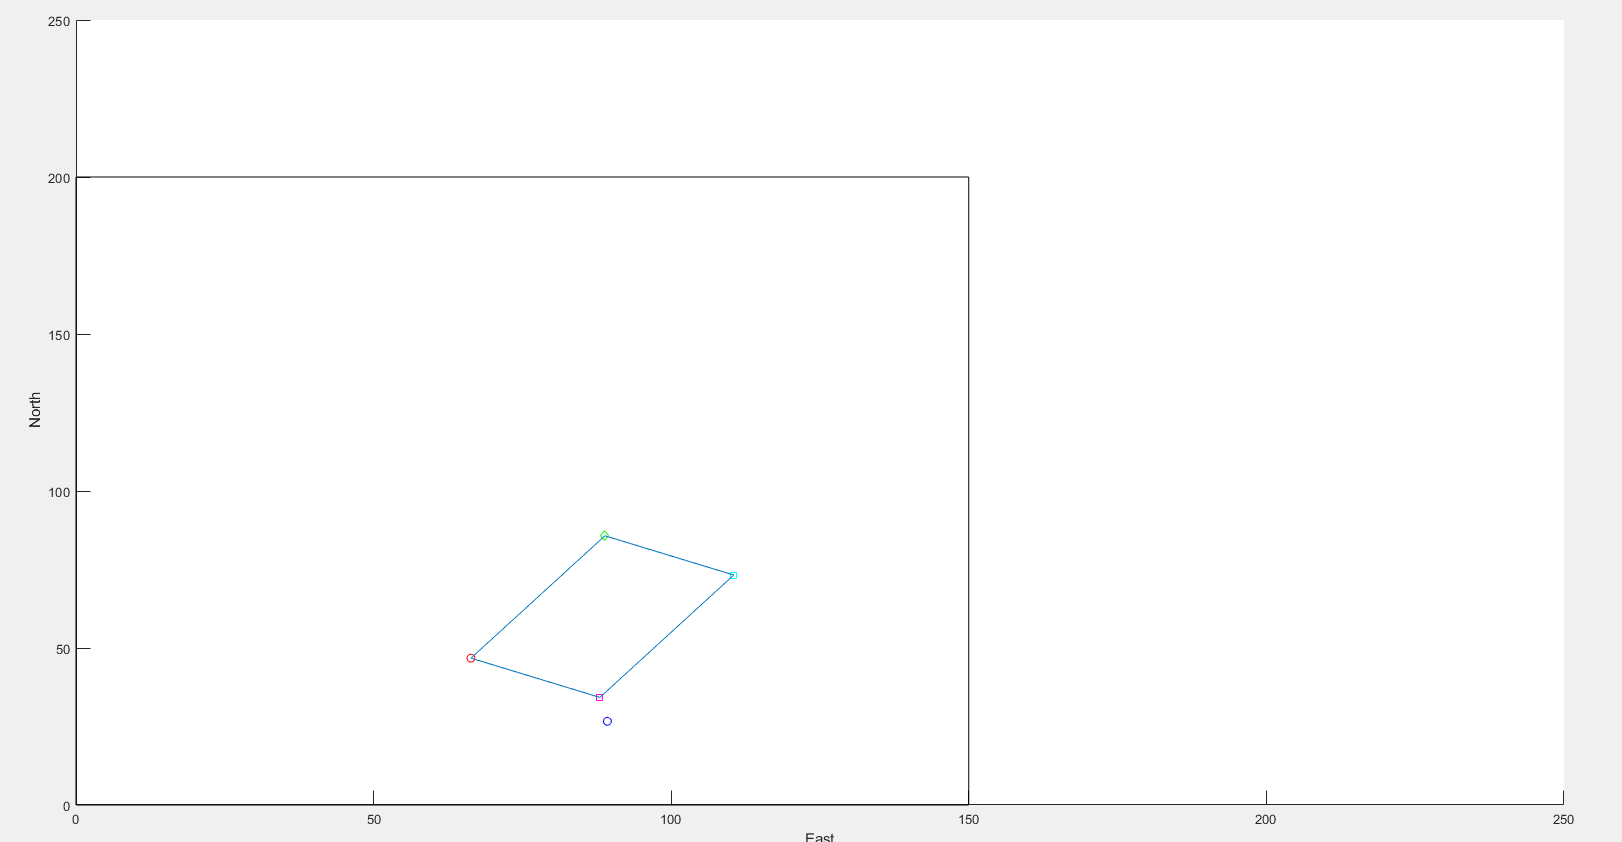
\includegraphics[scale = 0.3]{aread'interesse.png}}
                        \label{fig:area}
                \end{figure}
                    
                Il primo task pianificato è stato quello del \emph{positioning}.\\ 
                \\
                Nel file missionA.m viene fornito:\\
                \begin{itemize}
                    \item le coordinate in latitudine e longitudine  della variabile \emph{areaOfInterestCorner}, che ci indica la posizione di uno degli angoli dell'area
                    di interesse in cui può essere effettuata la missione;\\
                    \item la variabile \emph{surveyAreaCorner}, che rappresenta il vertice dell'area da scansionare;\\
                    \item le coordinate del punto di deploy \emph{initPoint}.\\ 
                \end{itemize}
                Mentre \emph{areaOfInterestCorner} indica sempre le stesse coordinate, \emph{surveyAreaCorner} e \emph{initPoint} sono parametrici.\\
                L'obiettivo di questo task consiste nella generazione dei riferimenti per il posizionamento del veicolo nel punto \emph{surveyAreaCorner}
                a partire dal punto di deploy.\\

                
                La fase \emph{diving} consiste semplicemente nell'immersione del veicolo dal punto di \emph{surveyAreacorner} al punto di inizio della vera e propria 
                scansione del fondale, tramite la generazione di riferimenti che vanno a modificare solo la componente nel vettore posizione relativa alla
                profondità, a seconda dell'altitudine da mantenere rispetto al fondale (parametro anch'esso variabile). Una volta completato questo task
                inizia la vera e propria survey che si suddivide in due macrotask:
                 \emph{'transect'} e \emph{'turn'}, che rappresentano rispettivamente la fase di transettatura e di virata.\\
                La nostra decisione è stata quella di effettuare la survey facendo muovere il veicolo sempre lungo il lato maggiore, sia esso in direzione 
                Est o in direzione Nord; i due casi sono evidenziati in figura \ref{fig:lati} :

                \begin{figure} [ht]
                    \caption{Possibili situazioni di configurazione dell'area d'interesse}
                    \makebox[\textwidth]{
                    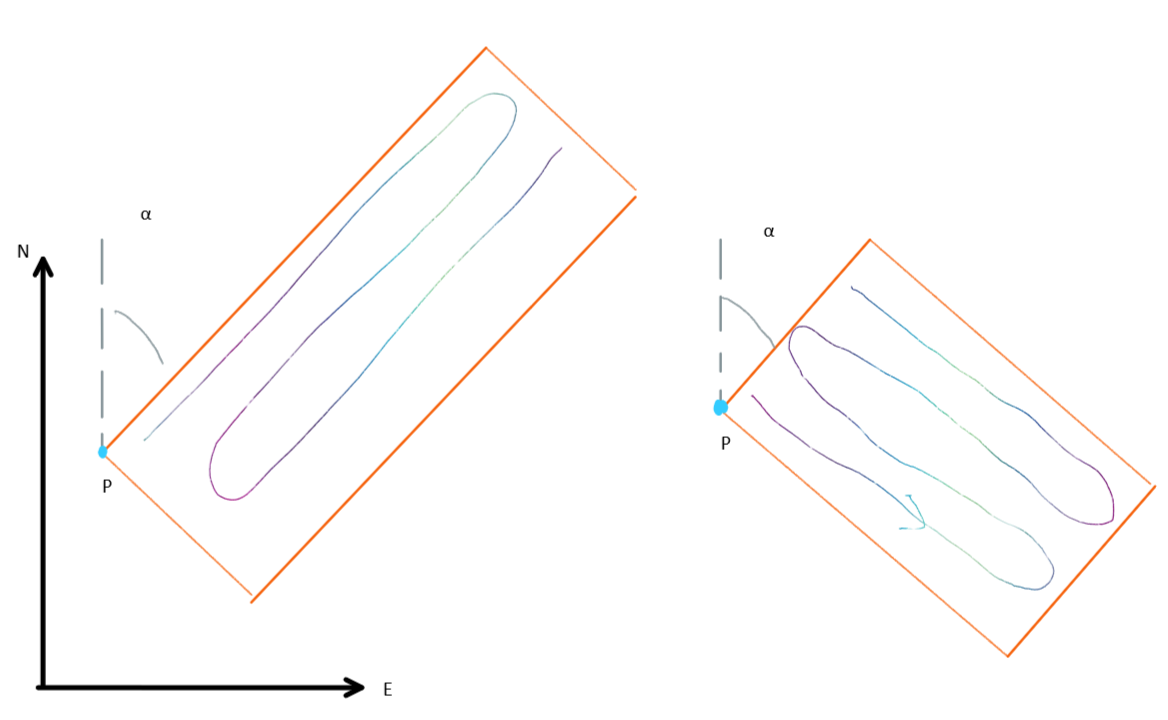
\includegraphics[scale = 0.3]{latisurvey}}
                    \label{fig:lati}
                \end{figure}

                Sono stati diversi i pro e i contro su cui si è ragionato per effettuare questa scelta.\\
                L'utilizzo del lato lungo per la survey è stato dettato dal fatto che in questa maniera avremmo potuto effettuare una survey 
                più veloce, in quanto avremmo diminuito il numero di virate che il veicolo avrebbe dovuto compiere. Le virate sono le traiettorie su cui il veicolo 
                deve rallentare, per varie cause (mantenimento in traiettoria più difficile da eseguire; forma allungata del veicolo, più 
                'debole' sullo sway; presenza di correnti sfavorevoli). Per questo motivo ne abbiamo largamente ridotto il numero.\\
                Il problema che però ci si era presentato in una seconda analisi è stato il fatto che avremmo potuto avuto difficoltà per il mantenimento
                del veicolo in traiettoria. Questo perché in una primissima fase di pianificazione iniziale 
                pensavamo di dare, per ogni transetto da compiere, solamente i riferimenti del punto iniziale e finale, andando a non definire il 
                comportamento del veicolo lungo tutta la fase di transettatura.\\
                Da qui, iniziando un ragionamento 
                sulla strategia da attuare in concomitanza col modulo \textit{Controllo}, siamo arrivati ad un valido compromesso: effettuando un controllo su traccia, 
                avremmo fornito lungo ogni transetto dei midwaypoints con riferimento di posizione, ad una distanza di 2.50m l'uno dall'altro, 
                ossia poco più della lunghezza del veicolo. Il veicolo, ogni qualvolta si sarà avvicinato all'i-esimo waypoint da raggiungere 
                entro un certo margine d'errore,
                riceverà il successivo riferimento di waypoint da raggiungere, continuando così sino alla fine del transetto attuale. 
                In questa maniera il problema che si era
                precedentemente presentato, di possibile non mantenimento della traiettoria dando solamente punto iniziale e finale (specialmente nel caso di transettatura 
                lungo il lato maggiore), è stato risolto.\\
                La parte implementativa riguardante il codice di generazione dei midwaypoints lungo il transetto è rimasta invariata anche durante le fasi di integrazione 
                con gli altri moduli: una volta preso in considerazione il lato maggiore di scansione, si generano offline i waypoints 
                e i relativi valori di riferimento, salvati tramite l'utilizzo in MATLAB di array multidimensionali. \\
                Ogni transetto è riferito utilizzando la terza dimensione (pagina) di tali array, indicizzata con la variabile $page$.
                Ogni riga all'interno di questa pagina rappresenta il riferimento di posizione dell'i-esimo waypoint e le colonne di ogni riga rappresentano le componenti 
                del vettore posizione. Quindi il numero di righe di ogni pagina rappresenta il numero di midwaypoints generati lungo ogni 
                transetto, mentre il numero di pagine rappresenta il numero di transettature da effettuare, che ovviamente varierà in base alla lunghezza del lato 
                con lunghezza 
                minore e al valore della variabile \emph{lineSpaceBetweenTransects}, che indica la distanza laterale tra un transetto e 
                il successivo.\\
                
                Arrivati a questo punto, terminate le fasi di esplorazione della survey, se tutto è quindi andato a buon fine avviene il \emph{surfacing}, che è il 
                task di riemersione dal punto di fine survey, durante il quale siamo andati a modificare solo la componente lungo Down del riferimento in posizione.\\
                L'ultima fase, coincidente con la prima a livello di logica implementativa, è la fase di \emph{positioning}, in cui il veicolo si dirige di nuovo 
                nel punto di deploy iniziale. La missione è dunque conclusa, e può essere visualizzata in figura \ref{fig:mission}.

                \begin{figure} [ht]
                    \caption{Esempio di traiettoria per l'intera missione}
                    \makebox[\textwidth]{
                    \includegraphics[scale = 0.3]{"plot\space trans\space più\space turn.png"}}
                    \label{fig:mission}
                \end{figure}

            \newpage
            \subsubsection{Dettagli aggiuntivi}
                Un'osservazione valutata nella fase di implementazione ha riguardato il caso in cui il lato di transettatura non fosse divisibile 
                senza resto rispetto alla distanza tra waypoints decisa. In tal caso si fornisce come ultimo punto di riferimento un punto aggiuntivo,
                giacente sul punto terminale del transetto, coincidente con l'inizio della virata;
                un esempio è mostrato nella figura \ref{fig:punti} :\\

                \begin{figure} [ht]
                    \caption{Suddivisione transetti in waypoints}
                    \makebox[\textwidth]{
                    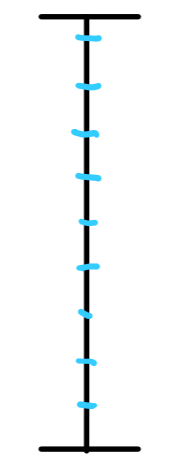
\includegraphics[scale = 0.3]{punti.png}}
                    \label{fig:punti}
                \end{figure}

                Un altro accorgimento ha riguardato poi il numero di transetti da compiere,
                dipendente dalla distanza orizzontale tra un transetto e l'altro \emph{lineSpaceBetweeenTransect}.
                A seconda del valore di questo parametro è possibile che 
                l'ultimo transetto si trovi al di fuori dei margini dell'area su cui effettuare la survey, come in figura \ref{fig:trans}.

                \begin{figure} [ht]
                    \caption{Gestione area da scansionare}
                    \makebox[\textwidth]{
                    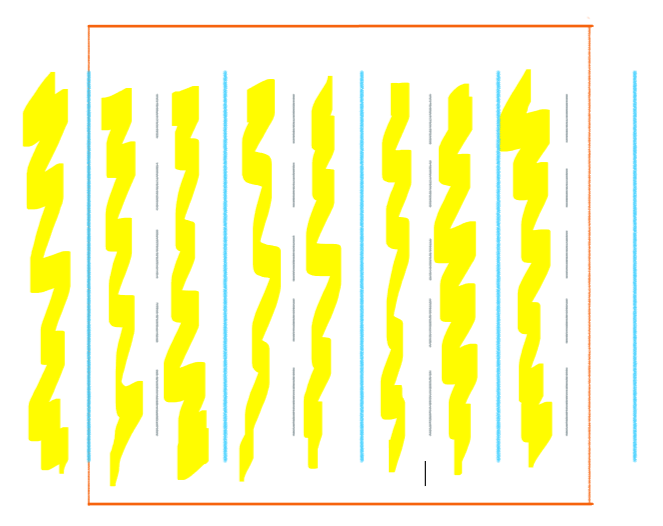
\includegraphics[scale = 0.3]{trans}}
                    \label{fig:trans}
                \end{figure}

                La decisione che abbiamo preso è stata quella di aggiungere una transettatura ulteriore solamente nel caso in cui la porzione di area ulteriore
                fosse più grande della metà di \emph{lineSpaceBetweenTransects},
                perchè questo significava lasciarla 'inesplorata' nell'ipotesi di scansione effettuata tramite sonar di raggio pari alla metà di tale valore.
                Nel caso in cui invece la traiettoria del transetto finale fosse abbastanza
                vicina al lato terminale dell'area, avremmo lasciato la generazione dei transetti invariata.\\

                L'ultima considerazione da sottolineare, per quanto riguarda l'esecuzione dei task di \emph{transect} e \emph{turn}, 
                è stata la decisione, presa in un secondo momento, di compiere le virate al di fuori dell'area di survey.
                Questa è stata dettata dal fatto che, dal momento che durante le virate solitamente non si prendono in considerazione le misure dei sonar,
                per evitare di perdere informazioni durante la manovra di virata abbiamo preferito lasciare tutte queste manovre al di fuori 
                dell'area di esplorazione effettiva, risultando una situazione come in figura \ref{fig:virata}.

                \begin{figure} [ht]
                    \caption{Considerazioni sulla gestione dell'area per le virate}
                    \makebox[\textwidth]{
                    \includegraphics[scale = 0.3]{"viratafuorisurvey\space (1).png"}}
                    \label{fig:virata}
                \end{figure}
                    
                Anche per quanto riguarda la fase di virata si era pensato un controllo su traccia tramite la generazione di riferimenti 
                di posa con midwaypoints intermedi, memorizzati in array multidimensionali in cui per ogni riga 
                è presente il riferimento dell'i-esimo midwaypoint corrispondente ed il numero di pagine corrisponde al numero di virate.
                L'unico accorgimento ulteriore è stato l'aver dovuto aggiungere un criterio di differenziazione per i casi di lato transettatura lungo
                su Nord e lato transettatura lungo su Est: nel primo caso le virate iniziano effettuando una rotazione oraria sul piano North-East con versore Down
                entrante nel piano, partendo dall'angolo $\alpha$
                di orientazione rispetto al Nord; nel secondo caso la prima virata avviene invece in senso antiorario e l'orientazione
                iniziale è quella di $\alpha$ gradi rispetto ad Est, quindi $\ 90 \degree + \alpha$ rispetto al Nord.\\
                A differenza di quanto avvenuto per i midwaypoints lungo i transetti, il cui codice generato offline è stato poi utillizzato nella survey fino alla fase 
                d'integrazione finale, questo approccio di generazione offline dei midwaypoints in virata è stato scartato per delle motivazioni che saranno spiegate 
                in seguito.\\

        \newpage
        \subsection{Macrotask d'emergenza}

            Per rappresentare eventuali situazioni di emergenza che possono verificarsi durante la missione abbiamo utilizzato degli altri stati.\\
            \\
            \emph{warning}: questo task si attiva solamente se il veicolo si trova disallineato (oltre un certo margine di errore) 
            rispetto alla traiettoria da seguire. La logica di base è che il 
            veicolo ritorni seguendo un moto traslazionale senza cambiare direzione di moto, dunque in questo caso abbiamo fornito come waypoint di riferimento 
            non quello immediatamente successivo al veicolo ma con indice aumentato, lasciando così al veicolo un margine di almeno 5m lungo la direzione di surge 
            per potersi ricondurre sulla traiettoria. La situazione è dunque quella di figura \ref{fig:disallineamento}.

            \begin{figure} [ht]
                \caption{Situazione di disallineamento da traiettoria desiderata}
                \makebox[\textwidth]{
                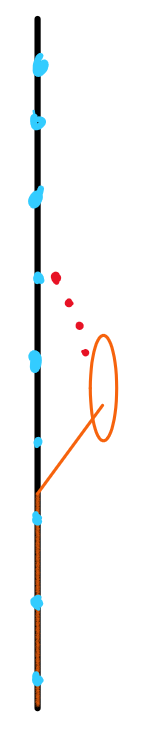
\includegraphics[scale = 0.3]{disalline.png}}
                \label{fig:disallineamento}
            \end{figure} 
                
            Un'altra situazione di emergenza è rappresentata dal task \emph{obstacle}: in questo task vengono generati i riferimenti opportuni in profondità, 
            qualora fosse presente un ostacolo. Per essere ritenuto tale, un oggetto deve presentare una variazione di fondale rilevante, maggiore di 0.5m,
            e le sue dimensioni devono superare i 2m lungo la direzione di surge del veicolo.\\ %TODO: figura?
            \\
            L'ultima emergenza è definita dal task \emph{abort}: questo task può essere richiamato secondo più situazioni di emergenza, ad esempio per
            una situazione di failsafe per danni strutturali. La nostra implementazione ha considerato la situazione in cui i motori del veicolo, 
            per malfunzionamento o altro, rimangono spenti per oltre un certo periodo di tempo.
            Altre ipotesi di failsafe possono essere quelle di danni ai sensori.

    \newpage
    \section{Logica di Stateflow}

        \subsection{Introduzione a Stateflow}

            \subsubsection{Stati}
                Stateflow è un toolbox di MATLAB che permette la modellazione e la simulazione di
                macchine a stati e diagrammi di flusso. \cite{stateflow}
                Stateflow viene integrato in uno schema Simulink con un blocco specifico, rappresentato in figura \ref{fig:chart} :\\
                All'interno della chart in Stateflow sono presenti diversi strumenti per implementare il flusso della macchina
                a stati, siano esse MATLAB function, simulink function, graphical function, truthTable... \\
                Il loro funzionamento sarà ripreso e chiarito al bisogno nella successiva 
                spiegazione dell'implementazione della nostra macchina a stati, alla base dello sviluppo dell'intero lavoro del nostro modulo.\\

                \begin{figure} [ht]
                    \caption{Chart in Stateflow}
                    \makebox[\textwidth]{
                    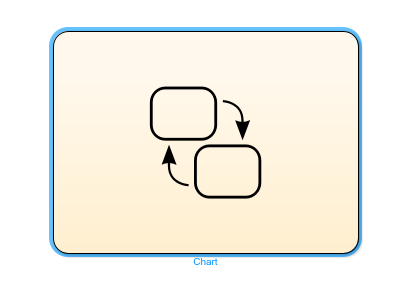
\includegraphics{chart.png}}
                    \label{fig:chart}
                \end{figure} 
                    
                Gli stati esclusivi del sistema sono rappresentati con una linea continua, mentre gli stati paralleli sono caratterizzati dalla linea tratteggiata, come in
                figure \ref{fig:escl} e \ref{fig:parallel} . 

                %TODO: accanto?
                \begin{figure} [ht]
                    \caption{Stati esclusivi nella macchina implementata}
                    \makebox[\textwidth]{
                    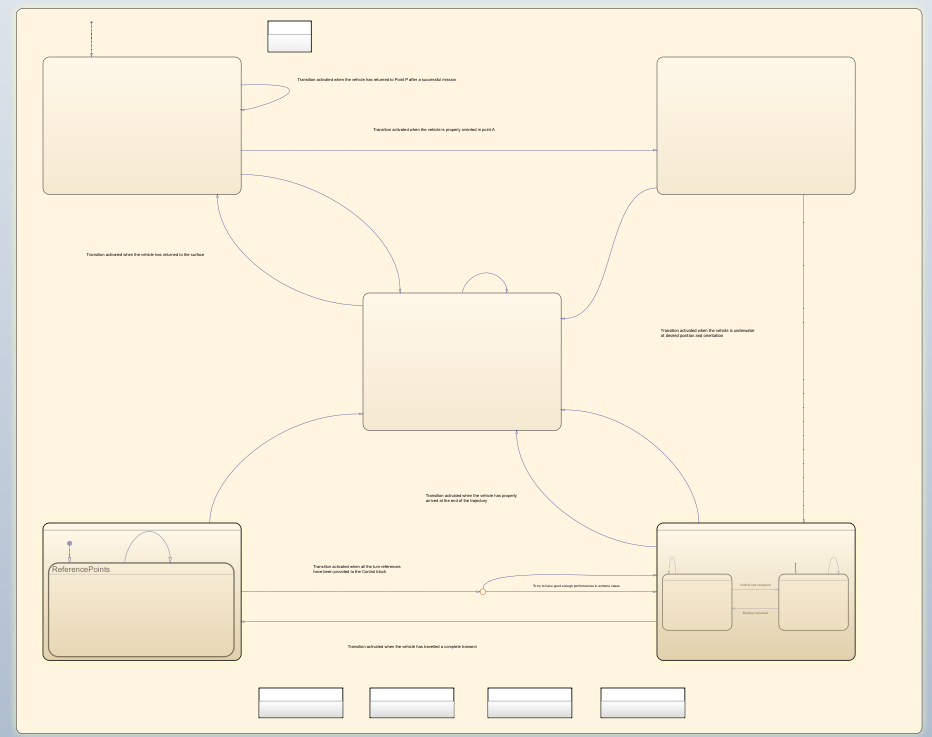
\includegraphics[scale = 0.3]{escl.png}}
                    \label{fig:escl}
                \end{figure} 
                    
                 
                \begin{figure} [ht]
                    \caption{Stati paralleli nella macchina implementata}
                    \makebox[\textwidth]{
                    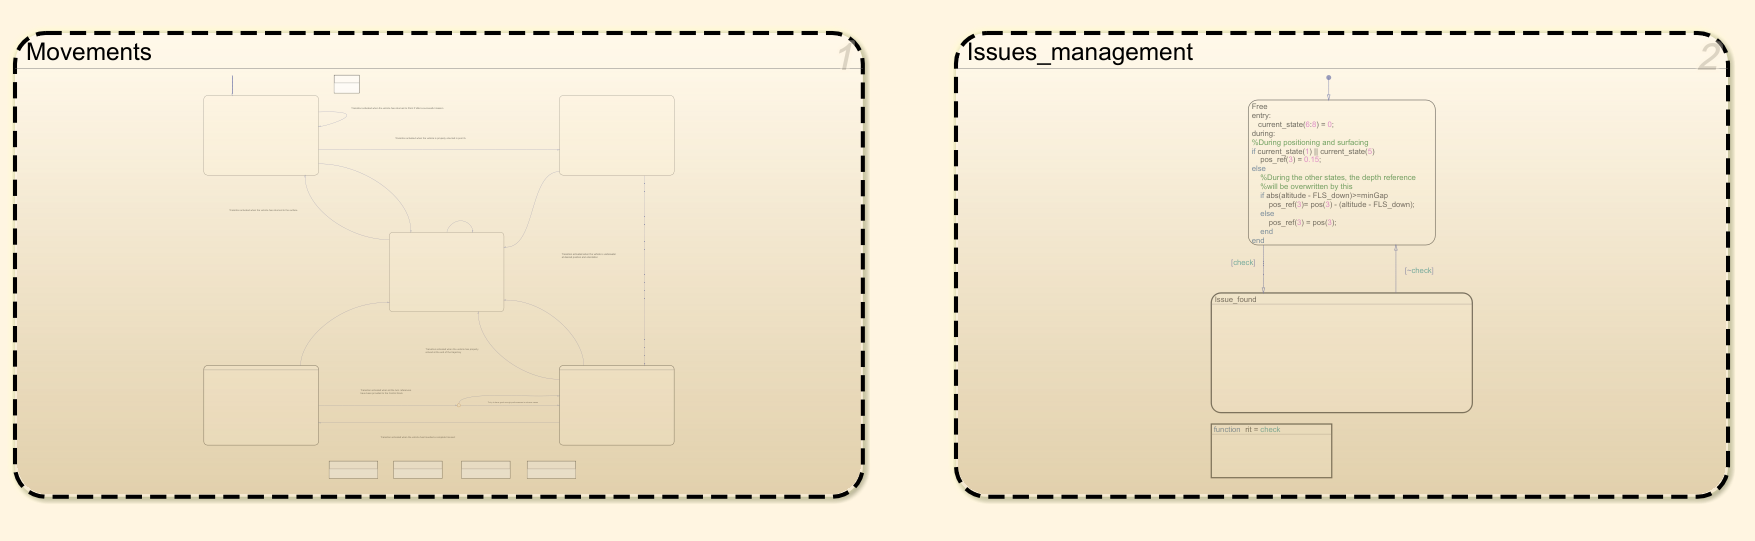
\includegraphics[scale = 0.3]{parallel.png}}
                    \label{fig:parallel}
                \end{figure}
            
            \subsubsection{Transizioni}
                
                Le transizioni sono rappresentate da frecce direzionate da uno stato ad un altro. \\
                Un caso particolare di transizione è quello della transizione di default in uno stato
                esclusivo, visibile in figura \ref{fig:default} :

                \begin{figure} [ht]
                    \caption{Transizione di default}
                    \makebox[\textwidth]{
                    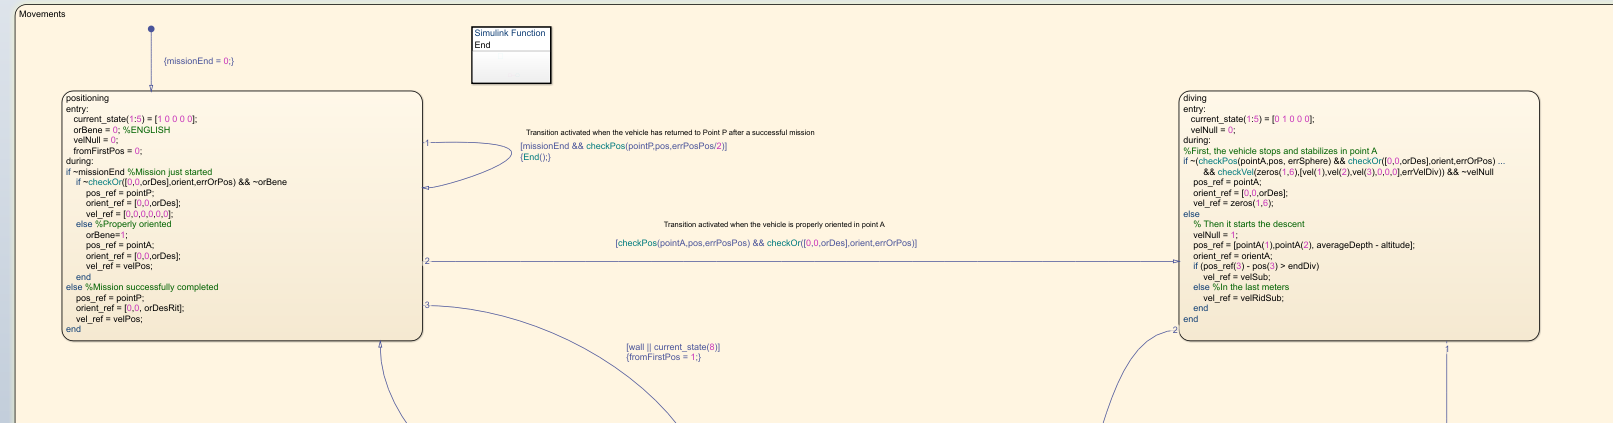
\includegraphics[scale = 0.3]{deftrans.png}}
                    \label{fig:default}
                \end{figure}
                    
                La transizione di default indica, fra tutti i blocchi esclusivi presenti all'interno di una subchart, quello in cui effettuare la prima transizione, 
                indicante quindi la condizione iniziale della macchina a stati.\\

            \subsubsection{Giunzioni}
                Le giunzioni (figura \ref{fig:joint} )sono rappresentate da cerchi cui possono giungere e partire più transizioni. Nel caso di più transizioni in uscita da una giunzione
                la sequenza di esecuzione viene determinata tramite un indice di priorità.\\

                \begin{figure} [ht]
                    \caption{Esempio d'uso di giunzioni}
                    \makebox[\textwidth]{
                    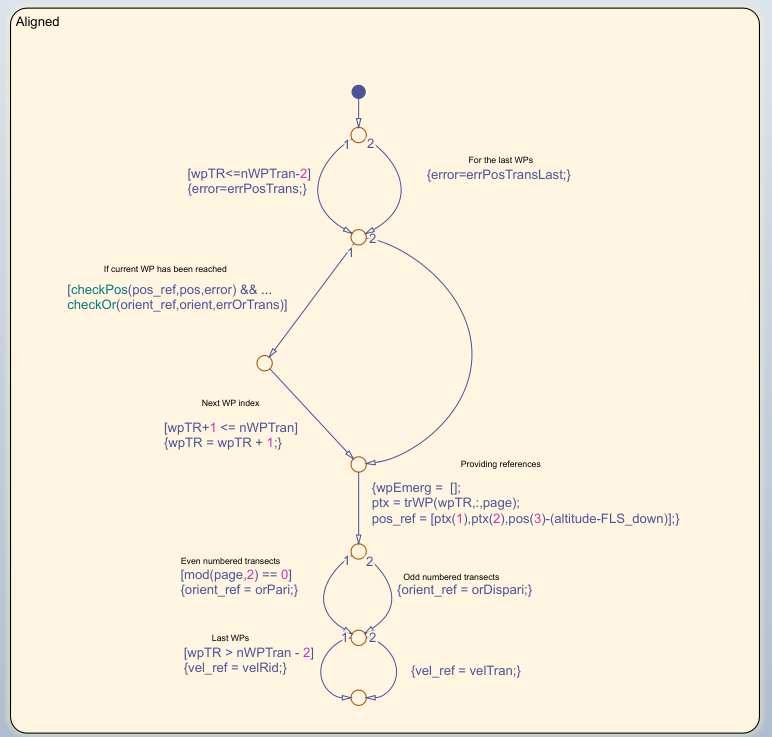
\includegraphics[scale = 0.3]{aligned.png}}
                    \label{fig:joint}
                \end{figure}

            
        \subsection{Tipi di azioni supportate per stati e transizioni}

            \subsubsection{Alcune azioni disponibili negli stati}

                \emph{entry}: esegue le operazioni non appena lo stato diventa attivo.\\
                \emph{during}: esegue l’azione quando lo stato è attivo, ad ogni ciclo di esecuzione.\\
                \emph{exit}: esegue le operazioni prime della transizione in uscita dallo stato.\\


                \begin{figure} [ht]
                    \caption{Entry condition in uno stato}
                    \makebox[\textwidth]{
                    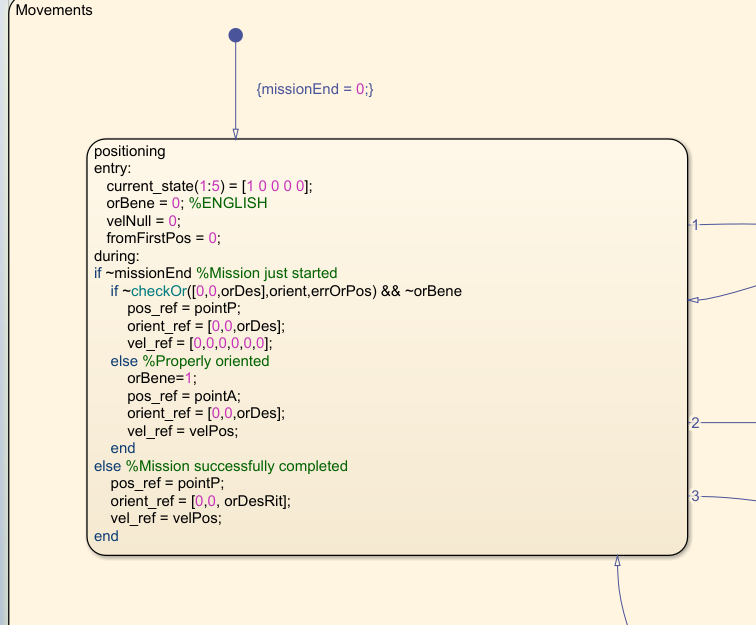
\includegraphics[scale = 0.3]{entri.png}}
                    \label{fig:entry}
                \end{figure}
                    
            \subsubsection{Tipi di azioni sulle transizioni:}

                \begin{figure} [ht]
                    \caption{Esempio di transizioni con condizioni}
                    \makebox[\textwidth]{
                    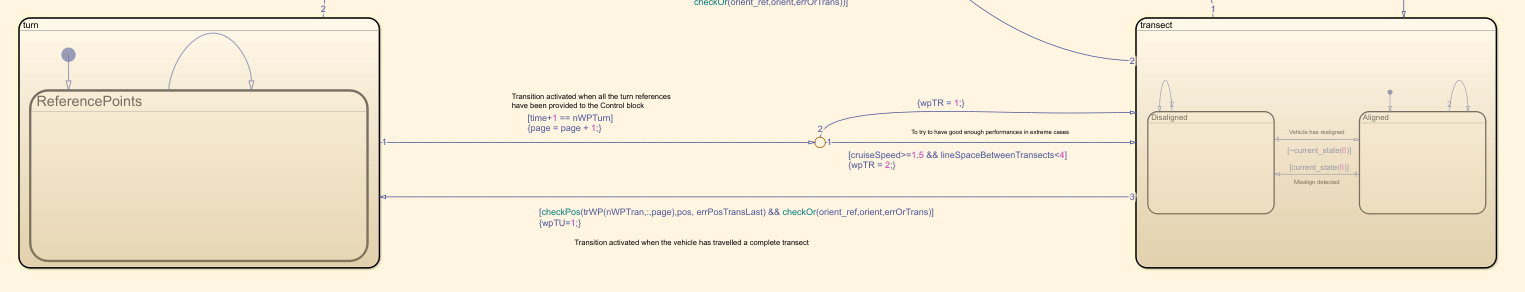
\includegraphics[scale = 0.3]{condit.png}}
                    \label{fig:my_label}
                \end{figure}
                    
                \textbf{Condition}\\
                La condizione è un’operazione booleana che determina se la transizione può essere effettuata oppure no. Condizioni possono essere:\\
                \begin{itemize}
                    \item espressioni booleane;\\
                    \item funzioni con valore di ritorno vero/falso o 0/1;\\
                    \item condizioni temporali;\\
                    \item eventi.
                \end{itemize}
                

                Vengono inserite sulle transizioni tra parentesi quadre.\\

                \textbf{Condition action}
                Sono operazioni messe tra parentesi graffe e vengono eseguite se la condizione è vera,
                prima che la destinazione della transizione sia raggiunta (stato o giunzione). \\
                A differenza di una transition action, l’operazione viene elaborata anche nel caso in cui non sarà possibile effettivamente effettuare
                la transizione.\\

    \newpage
    \section{Implementazione della nostra macchina a stati}
        Verranno descritti ora la politica di gestione della nostra macchina a stati e il codice al suo interno, per rendere più chiaro e comprensibile il suo funzionamento e
        l'efficacia del suo utilizzo.

        \begin{figure} [ht]
            \caption{Subchart della macchina a stati implementata}
            \makebox[\textwidth]{
                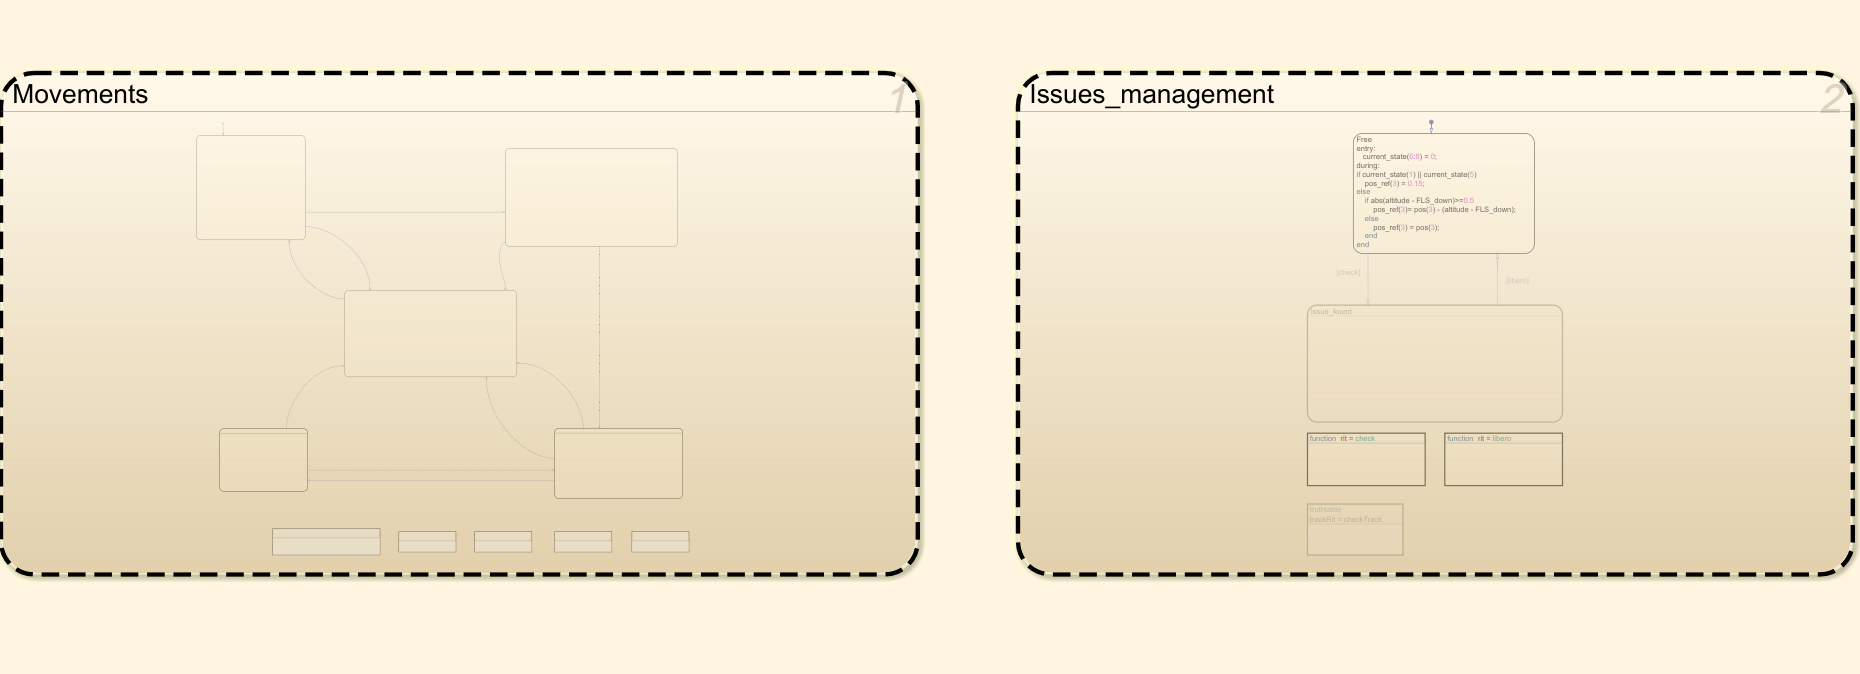
\includegraphics[scale = 0.3]{macchstati.png}}
                \label{fig:macchina}
        \end{figure}
            
        Come si può ben vedere nella figura \ref{fig:macchina} , la nostra macchina a stati comprende due subcharts principali: 
        \begin{itemize}
            \item \textbf{Movements}
            \item \textbf{Issues\_Management}.
        \end{itemize}
        
        Le due Subcharts sono tratteggiate, ad indicare sono trattate come stati paralleli e che quindi vengono attivati contemporaneamente. 

        \subsection{Subchart Movements}

            La subchart  \emph{Movements} comprende i cinque task nominali sopra descritti, implementati come stati esclusivi: ricodiamo che la loro attivazione viene
            segnalata settando il relativo bit tra i primi cinque presenti nel vettore \emph{current\_state}.
            \\
            La default transition all'interno della subchart si trova 
            sullo stato \emph{positioning}, così che lo stato iniziale in cui si trova la nostra macchina a stati sia quello di posizionamento. In contemporanea, 
            nel blocco  \emph{Issues\_management} è presente una default transition sullo stato \emph{Free}, che rappresenta l'assenza di situazioni di emergenza;
            appena si attiva l'intera macchina a stati sono attivi quindi gli stati \emph{positioning} e \emph{Free}. \\
            Per quanto riguarda le emergenze la macchina a stati sarà settata a \emph{Free} sino a quando non si presenta una situazione che necessita di attenzioni:
            a quel punto viene settato \emph{current\_state} in maniera da avere bit a 1 in posizione relativa al 
            tipo di emergenza rilevata, con conseguente transizione nel relativo stato.\\
            \\
            
            \begin{figure} [ht]
                \caption{Stato di positioning}
                \makebox[\textwidth]{
                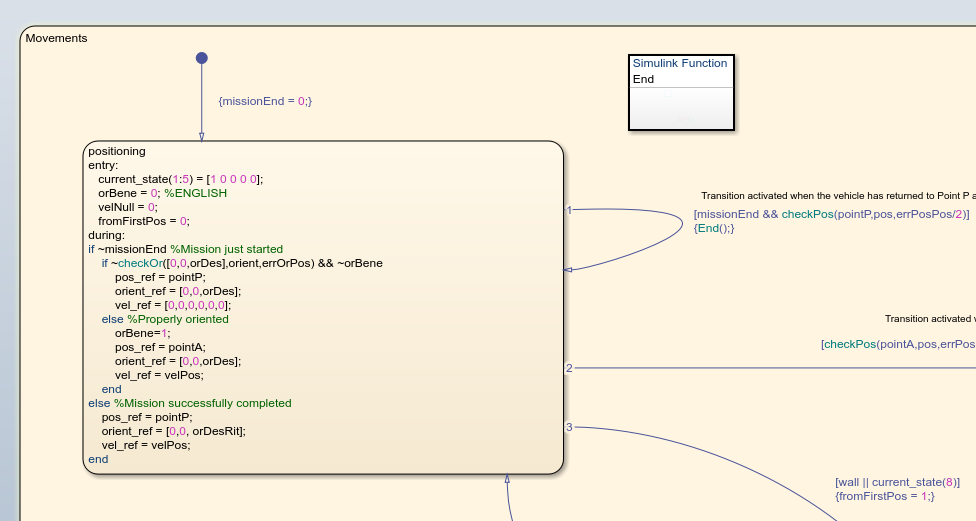
\includegraphics[scale = 0.3]{positioning.png}}
                \label{fig:positioning}
            \end{figure}
                
            Il primo stato nel blocco \emph{Movements} è \emph{positioning} (figura \ref{fig:positioning} ), caratterizzato da una default transition, 
            avente una condition action che setta il flag \emph{missionEnd} a 0. 
            \\
            Appena si entra nel blocco, quello che viene fatto è settare \emph{current\_state} al valore $[1 0 0 0 0 0 0 0]$. 
            Durante il posizionamento il modulo effettua un check su orientazione e velocità, per gestire il quale utilizziamo delle variabili flag:
            essendo all'inizio nel caso di orientazione 
            e velocità desiderate non raggiunte, le variabili vengono settate a 0; successivamente si effettua il controllo sopra citato. Innanzitutto, se $\emph{missionEnd} = 0$
            siamo in condizione di missione iniziata; la funzione di check fa sì che il blocco continui ad inviare sempre gli stessi valori di riferimento per posizione,
            orientazione e velocità relativi a \emph{initPoint} fintanto che il veicolo non si è stabilizzato intorno al punto di deploy orientandosi lungo la congiungente
            tra esso ed il punto \emph{surveyAreaCorner}.
            Una volta accaduto ciò, il veicolo inizerà a spostarsi per portarsi da \emph{initPoint} a \emph{surveyAreaCorner}.\\
            Per quanto riguarda i riferimenti di posizione e di orientazione, inizialmente si era pensato di dare solamente posizione e orientazione finali 
            del veicolo, ma successivamente, in fase di implementazione, il modulo \textit{Controllo} ha richiesto dei riferimenti che permettessero
            un controllo più 'discretizzato' per le  singole manovre da compiere: presupponendo che il veicolo sia
            calato in acqua con orientazione nota e pari all'angolo $\alpha$ rispetto all'asse Nord, e conoscendo la distanza tra l'origine e il punto P
            (\emph{initPoint}) e l'origine e il punto A (\emph{surveyAreacorner}), ne ricaviamo un riferimento di orientazione tale che
            il veicolo possa orientarsi lungo direzione e verso del vettore differenza PA, valore che in figura \ref{fig:sppos} è l'angolo $\gamma$. 

            
            \begin{figure} [ht]
                \caption{Situazione d'esempio durante il posizionamento}
                \makebox[\textwidth]{
                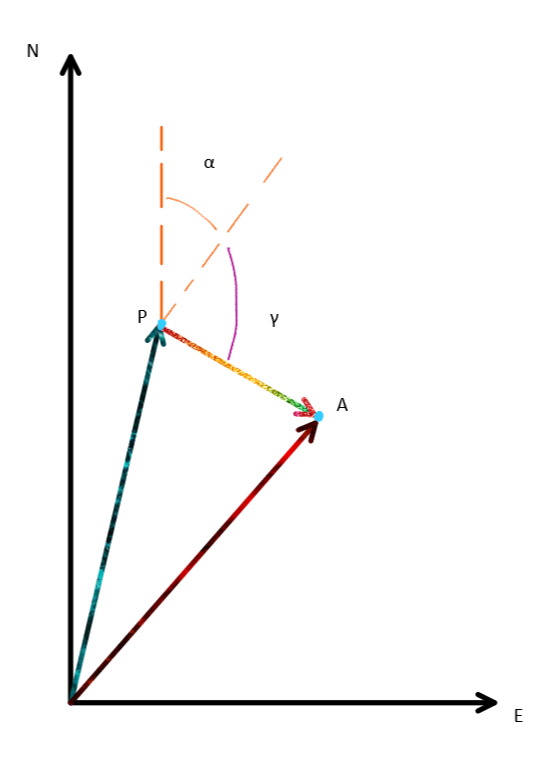
\includegraphics[scale = 0.3]{spiegpositioning.png}}
                \label{fig:sppos}
            \end{figure}

            Avvenuta la corretta orientazione del veicolo, il veicolo si dirige nel punto \emph{surveyAreaCorner}. \\
            Una volta che arriva all'interno dell'area sferica di raggio 1.50m centrata in tale punto, si effettua la transizione allo stato \emph{diving} di figura \ref{fig:diving} : 

            \begin{figure} [ht]
                \caption{Stato di diving}
                \makebox[\textwidth]{
                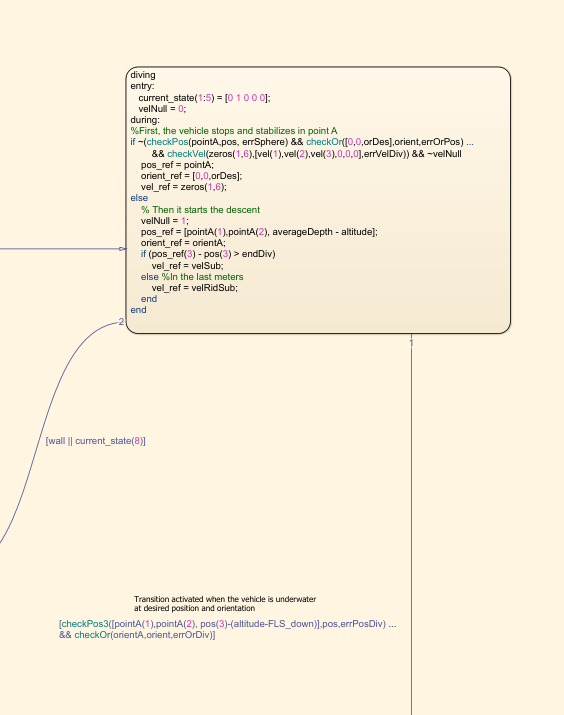
\includegraphics[scale = 0.3]{diving.png}}
                \label{fig:diving}
            \end{figure}

            Durante l'entry si setta \emph{current\_state} con bit 1 in posizione 2 e, prima di entrare  nella vera e propria fase di immersione, 
            si fa un check di velocità utilizzando, come nello stato positioning, una variabile di flag. Considerando dei margini di errore accettabili,
            finché il veicolo non arriva nel punto desiderato con orientazione desiderata e velocità nulla, 
            non avviene il cambio di riferimento in profondità. Si è decisa questa implementazione per assicurarci
            che il veicolo sia ben posizionato e fermo sul punto di immersione, così da minimizzare gli errori.\\
            Una volta che il check è andato a buon fine, si inizia l'immersione e vengono passati i nuovi riferimenti
            di posizione (con la nuova profondità) e orientazione del veicolo. \\
            A fine immersione il veicolo si fermerà e, raggiunto il punto di inizio survey con posizione
            e orientazione desiderate, può iniziare la vera e propria scansioe del fondale tramite le fasi di transettature e virate, visualizzabili in figura \ref{fig:transect} .

            \begin{figure} [ht]
                \caption{Stato di transect}
                \makebox[\textwidth]{
                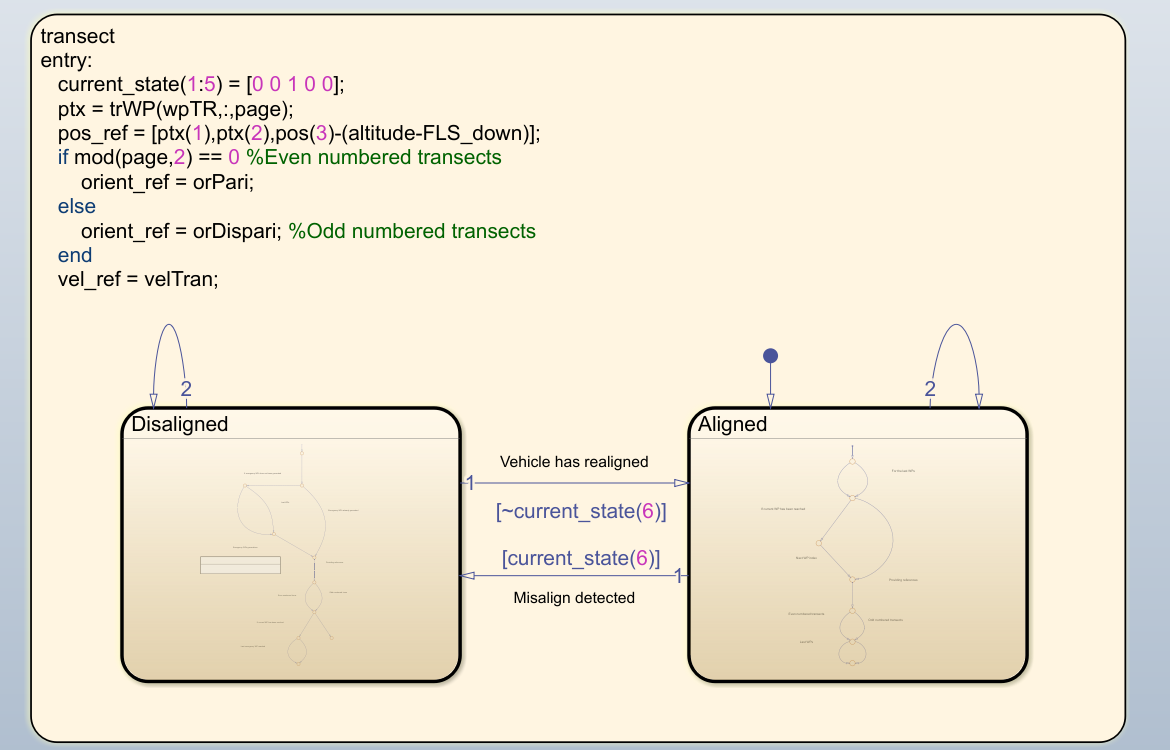
\includegraphics[scale = 0.3]{transect.png}}
                \label{fig:transect}
            \end{figure}

            Nell'entry di \emph{transect}, come in ogni stato, la prima cosa che si fa è settare il corretto bit di \emph{current\_state}. Si comincia poi a fornire i riferimenti
            relativi al primo waypoint da raggiungere.
            Ad inizio scansione, il riferimento sarà relativo alla prima riga della prima pagina della matrice contenente i waypoints. Si utilizzano in seguito gli indici in figura \ref{fig:param} .

            \begin{figure} [ht]
                \caption{Parametri per gestione delle matrici di waypoint}
                \makebox[\textwidth]{
                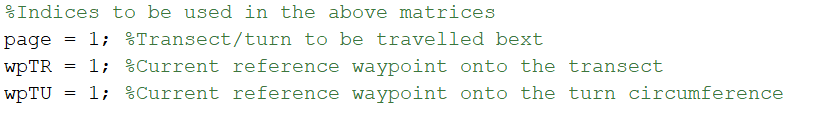
\includegraphics[scale = 0.3]{param.png}}
                \label{fig:param}
            \end{figure}

            Come si può vedere in figura \ref{fig:pages} , transetti e virate sono indicizzati secondo la stessa variabile \emph{page}, andando poi ad utilizzare un ulteriore
            indice per indicare quale waypoint si sta correntemente fornendo al blocco \textit{Controllo}.
            
            \begin{figure} [ht]
                \caption{Gestione matrici nel passaggio a nuovo transetto}
                \makebox[\textwidth]{
                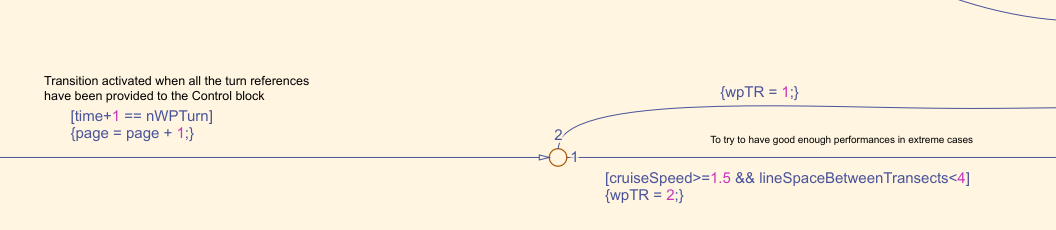
\includegraphics[scale = 0.3]{pages.png}}
                \label{fig:pages}
            \end{figure}
                
            L'unico accorgimento preso durante la transizione da \emph{turn} a \emph{transect},
            per cercare di mantenere performance migliori, è stato quello di fornire non il primo waypoint sul transetto ma il secondo.\\
            Nell'entry di questo blocco diamo anche il riferimento di orientazione per distinguere i casi di transetto di indice dispari, 
            su cui il veicolo deve essere orientato con angolo di imbardata $\alpha$ rispetto all'asse Nord, e di indice pari, su cui il veicolo deve orientarsi secondo
            $ \alpha + 180\degree $, poichè deve andare in direzione opposta al transetto precedente.\\
            Lungo il transetto, considerando un certo margine di errore su surge e sway, ci si può trovare allineati, con attivazione del sottostato \emph{Aligned}, 
            o disallineati, con attivazione del sottostato \emph{Disaligned}.
            \\
            \\
            All'interno del blocco transect la default transition è settata su \emph{Aligned}, in figura \ref{fig:aligned} .

            \begin{figure} [ht]
                \caption{TODO}
                \makebox[\textwidth]{
                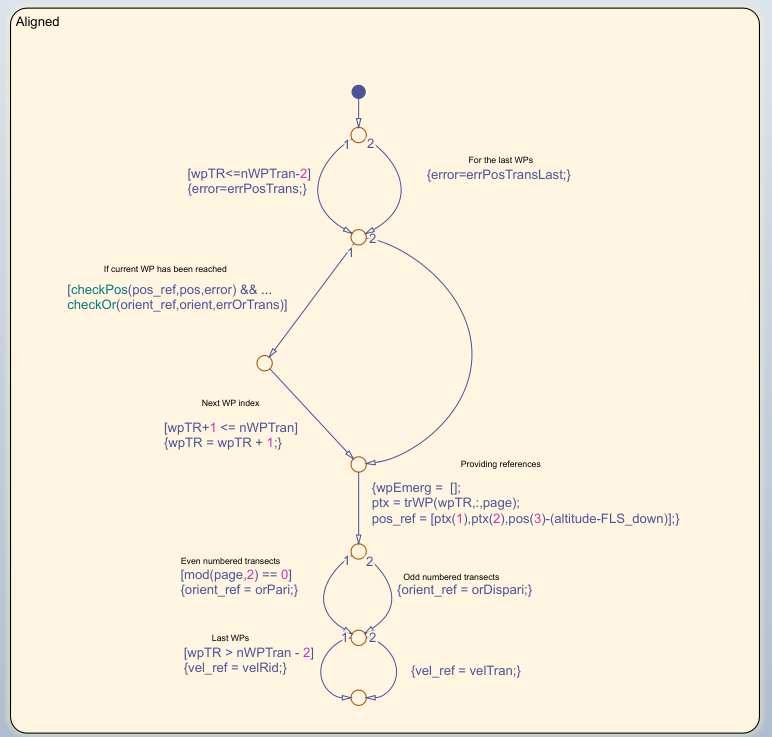
\includegraphics[scale = 0.3]{aligned.png}}
                \label{fig:aligned}
            \end{figure}

            E' poi presente una check function su posizione e orientazione: finchè tali riferimenti non sono raggiunti, il check non è soddisfatto, quindi si procedere a
            inizializzare la matrice di waypoint di emergenza ad una matrice vuota e si continua a dare lo stesso waypoint di riferimento.\\
            Nel caso in cui invece il check dia esito positivo, finchè l'indice riga del waypoint successivo è inferiore o uguale al numero di waypoints \emph{nWPTran}, 
            si procede a fornire il waypoint successivo. Un controllo aggiuntivo determina se l'indice di riga corrisponde al terzultimo
            waypoint di riferimento, quindi ad almeno 5 m di distanza dall'ultimo, e in caso sia così si va ad indicare al veicolo di 
            rallentare, portandosi ad una velocità di virata di 0.2m/s. Si è scelto un margine di frenata 
            di 5m poichè, essendo la velocità di crociera parametrica, vogliamo esser sicuri che lo spazio di frenata sia tale da permettere al veicolo di arrivare
            in curva con la velocità ridotta desiderata. \\ 

            Le funzioni \emph{checkPos} e \emph{checkOr} sono le stesse sia per \emph{transect} che per \emph{turn}, utilizzando però valori numerici e margini differenti.\\
            Per quanto riguarda la funzione \emph{checkPos}, notiamo in figura \ref{fig:condit} che
            nella fase di transettatura accetta un margine di errore su surge e sway di 1m: questo significa che quando distiamo meno 
            di 1m dal waypoint di riferimento, forniamo già il riferimento relativo al punto successivo, sia esso sempre sul transetto o in virata (dopo un cambio di stato).
            Per gli ultimi waypoint sui transetti il margine sulle coordinate di surge e sway da rispettare è ridotto a 0.50m, poiché
            vogliamo che il veicolo sia già ben posizionato e orientato prima di procedere in curva. \\            

            \begin{figure} [ht]
                \caption{Condizioni di transizione da virata a transetto e viceversa}
                \makebox[\textwidth]{
                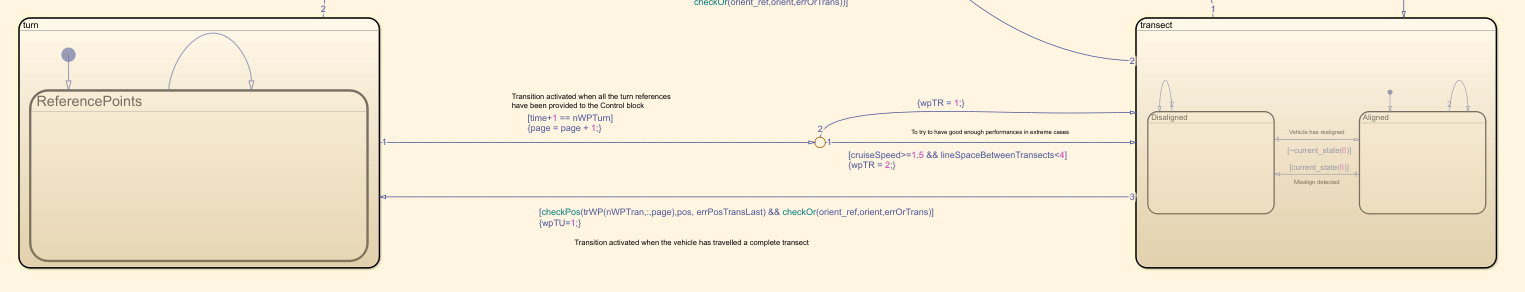
\includegraphics[scale = 0.3]{condit.png}}
                \label{fig:condit}
            \end{figure}



            Arrivati nel blocco \emph{turn} (figura \ref{fig:turn} ), la prima cosa che si fa nell'entry è ovviamente settare il bit relativo nel \emph{current\_state}. 

            \begin{figure} [ht]
                \caption{Stato di turn}
                \makebox[\textwidth]{
                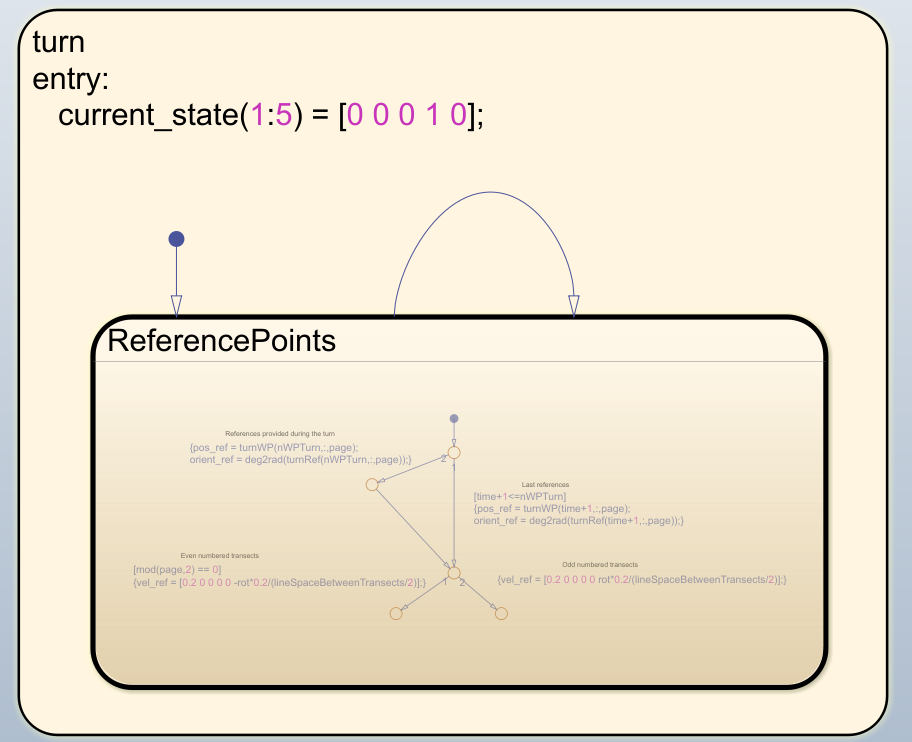
\includegraphics[scale = 0.3]{turn.png}}
                \label{fig:turn}
            \end{figure}

            Per quanto riguarda questo stato, vi è stata un'evoluzione della sua implementazione durante le varie fasi del lavoro ed è utile menzionarle tutte.\\ \\
            Inizialmente avevamo realizzato una funzione del tutto analoga a quella di generazione dei waypoint dei transetti: quindi utilizzavamo delle matrici multidimensionali, 
            una per quanto riguarda le posizioni di riferimento ed una per le orientazioni di riferimento da passare. L'angolo di $180 \degree$ della semicirconferenza
            rappresentante la curva sarebbe stato diviso in cinque parti e per ogni arco di circonferenza spazzato sarebbero stati forniti riferimenti di posizione e 
            orientazione del relativo midwaypoint. \\
            Durante la fase d'implementazione il modulo \emph{Controllo} ha riportato la necessità di utilizzare come riferimento il solo centro della curva di virata
            in maniera tale da calcolarsi la distanza laterale di ogni punto della virata rispetto al centro e poterla tenere al valore del raggio di curvatura,
            effettuando quindi principalmente un controllo sullo
            sway. \\
            Dopo aver effettuato numerose prove in cui la curva veniva eseguita sufficientemente bene senza disallineamenti eccessivi, si è notato che durante la
            primissima parte della curva non riusciva ad orientarsi perfettamente. Sapevamo bene di non necessitare di 
            un inseguimento di traiettoria su curva che fosse irrealisticamente preciso, anche perchè in curva non avvengono rilevazioni per il vero task di scansione del fondale,
            ma su consiglio e richiesta degli altri moduli abbiamo pensato ad un metodo che potesse essere più efficiente da questo punto di vista. Il modulo \emph{Controllo} è
            poi giunto alla conclusione (d'implementazione finale) di utilizzare un passaggio di riferimenti temporizzato in base alla loro frequenza di lavoro,
            utilizzando quindi un timer come quello di figura \ref{fig:timer} .\\ 
            Con questo nuovo metodo (figura \ref{fig:virate} ) abbiamo ottenuto un inseguimento più accurato della curva, anche in casi di dimensioni più ristrette, seppur con qualche perdita di precisione
            in casi estremi. 

            \begin{figure} [ht]
                \caption{Gestione riferimenti in virata}
                \makebox[\textwidth]{
                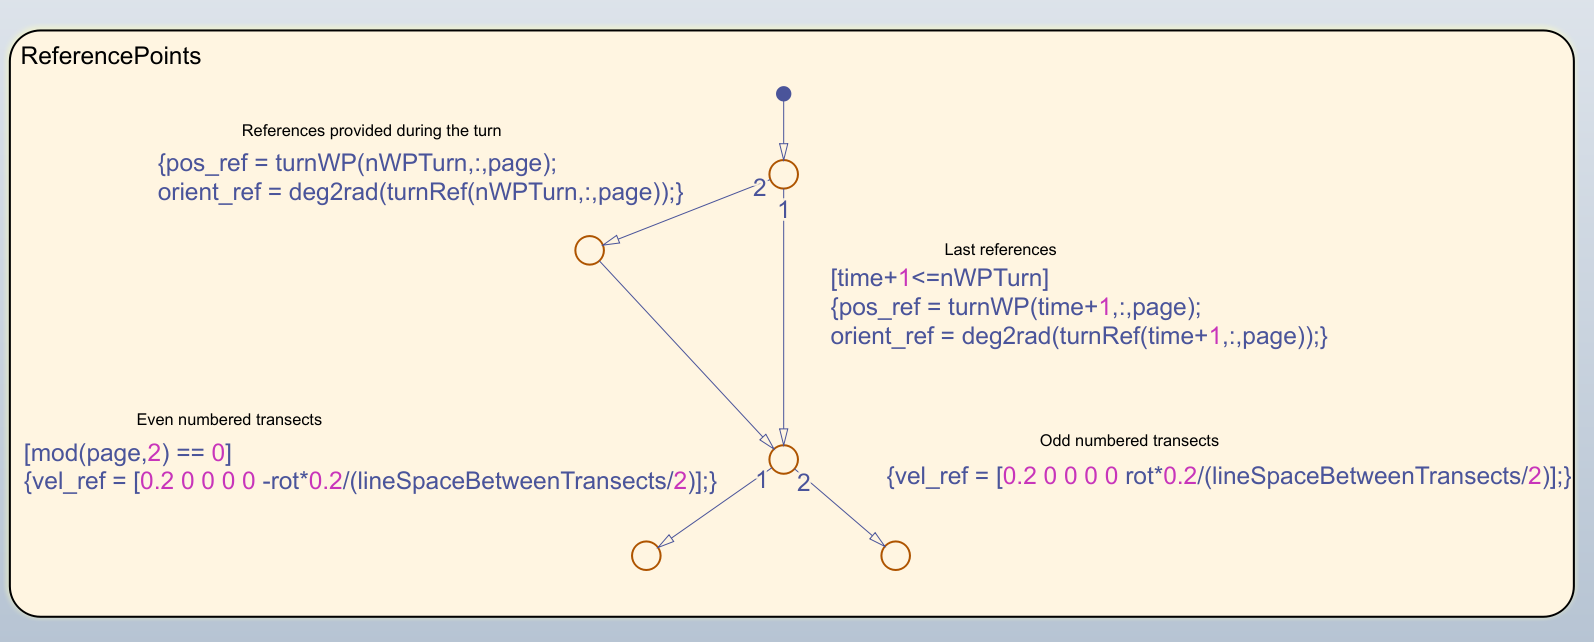
\includegraphics[scale = 0.3]{virate.png}}
                \label{fig:virate}
            \end{figure}

            In questo caso abbiamo mantenuto le matrici per salvare i waypoints di riferimento, andando poi a fornirli al 
            modulo \emph{Controllo} volta per volta senza effettivamente effettuare un check sul raggiungimento dei riferimenti.

            \begin{figure} [ht]
                \caption{Timer implementato}
                \makebox[\textwidth]{
                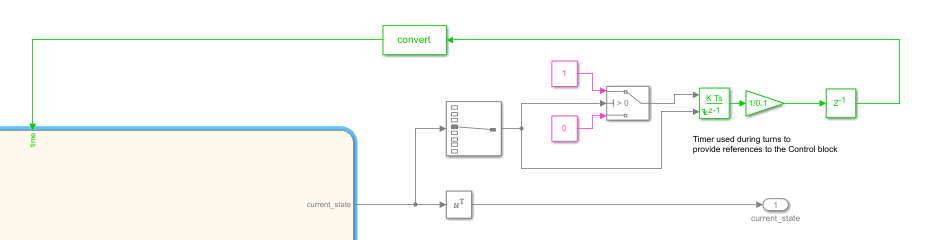
\includegraphics[scale = 0.3]{timer.png}}
                \label{fig:timer}
            \end{figure}

            
            In uscita al current state è stato quindi inserito un blocco selettore indicante la quarta posizione del vettore \emph{current\_state}.
            Quando siamo in fase di turn si attiva questa funzione di timer attraverso un blocco integratore 
            discreto attraverso il quale si ottiene il parametro per indicizzare la matrice di riferimenti in virata, in maniera tale da campionare la curva e 
            fornire il riferimento ogni 0.1s (frequenza di campionamento del controllore).\\
            Tramite l'uso di un delay e del blocco convert ci assicuriamo di indicizzare la matrice tramite variabili intere e di non creare loop algebrici. 

            \begin{figure} [ht]
                \caption{Generazione di riferimenti in base al raggio di virata}
                \makebox[\textwidth]{
                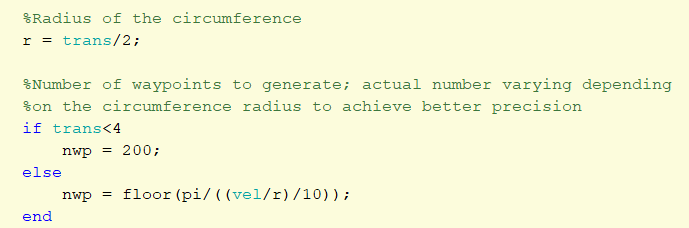
\includegraphics[scale = 0.3]{raggio.png}}
                \label{fig:raggio}
            \end{figure}


            Dopo una serie di prove di tipo trial and error, ci siamo resi conto che per ottenere dei buoni inseguimenti di traiettoria in curva bastava utilizzare un numero
            di waypoint variante in base al raggio di circonferenza e alla velocità angolare del veicolo (figura \ref{fig:raggio} ).\\
            Abbiamo differenziato solo il caso di raggi di curvatura minori di 2m, per i quali forniamo un 'sovrannumero' (200) 
            di waypoints di riferimenti in curva, per cercare di mantenere performance omogenee anche in casi estremi di esplorazione di 
            fondale con transetti a distanze molto ravvicinate e velocità elevate.\\
            Nel blocco \emph{ReferencePoints}, come precedentemente detto, non è presente un check di posizione e orientazione, perchè l'aver generato dei riferimenti 
            abbastanza fitti risolve il problema di inseguimento 'qualitativo' della traiettoria circolare. L'unico accorgimento resosi necessario è stato riguardante il
            riferimento di velocità, poichè sui transetti pari la velocità angolare di yaw deve essere positiva, mentre sui transetti dispari negativa alla precedente.\\
            Ogni volta che si è finito di compiere la virata, quindi quando vale la condizione  $time + 1 == nWPTurn$ in figura \ref{fig:time}, si resettano gli indici prima di passare al transetto successivo.

            \begin{figure} [ht]
                \caption{Uso della variabile 'time'}
                \makebox[\textwidth]{
                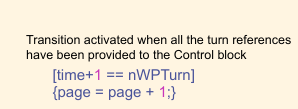
\includegraphics[scale = 0.3]{time.png}}
                \label{fig:time}
            \end{figure}

            Un ultimo stato è quello di riemersione, \emph{surfacing} in figura \ref{fig:surf} : è presente una transition verso lo stato di riemersione per ogni stato della subchart \emph{Movements},
            perché si potrebbe decidere di riemergere da qualsiasi degli stati precedentemente discussi.\\
            La riemersione viene infatti attivata sia in caso 
            di failsafe, danni strutturali, che in caso di ostacoli compromettenti la missione, tramite la parte di modulo rappresentato in figura \ref{fig:wall} .

            \begin{figure} [ht]
                \caption{Stato di surfacing}
                \makebox[\textwidth]{
                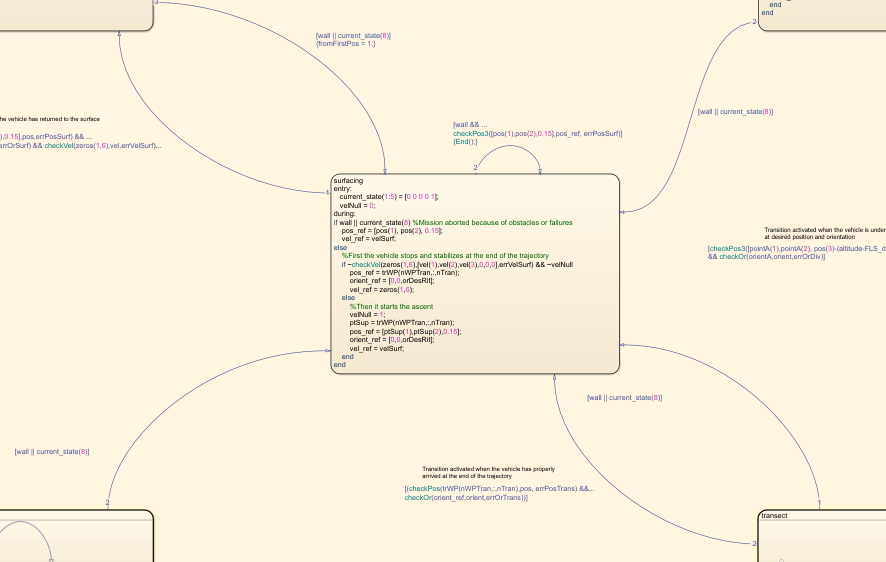
\includegraphics[scale = 0.3]{surf.png}}
                \label{fig:surf}
            \end{figure}

            Quando si entra nello stato \emph{surfacing} viene settato il bit relativo e inizializzata una variabile flag per controllo sulla velocità.
            Per prima cosa infatti si controlla che il veicolo si mantenga sul punto corrente variando solo la sua profondità.

            \begin{figure} [ht]
                \caption{Prime condizioni nello stato di emersione}
                \makebox[\textwidth]{
                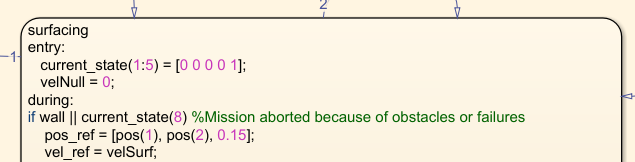
\includegraphics[scale = 0.3]{wall.png}}
                \label{fig:wall}
            \end{figure}

            Vi è una transition aggiuntiva da \emph{transect} a \emph{surfacing} nel caso di completamento della missione.\\ 
            Si compie un ultimo check di posizione e orientamento e, quando siamo all'interno di sfera centrata sull'ultimo waypoint dell'ultimo transetto e di raggio 1m,
            viene effettuata la transizione e si attiva la riemersione: il veicolo dapprima si fermerà in tale area e in seguito procederà a riemergere, come indicato dalla transizione
            di figura \ref{fig:emer}.

            \begin{figure} [ht]
                \caption{Esempio di attivazione della riemersione}
                \makebox[\textwidth]{
                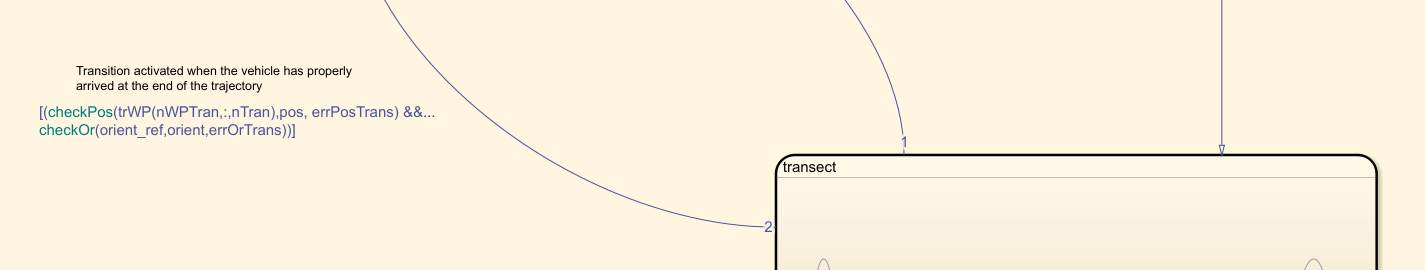
\includegraphics[scale = 0.3]{eme.png}}
                \label{fig:emer}
            \end{figure}
                
            Analogamente, se la missione è andata a buon fine il veicolo comincerà la vera e propria emersione solo dopo essersi fermato. Per questo, se la velocità 
            non è nulla si continua a fornire l'ultimo riferimento di posizione e si indicherà al veicolo di arrestarsi, seguendo quanto indicato in figura \ref{fig:emer2} .\\

            
            \begin{figure} [ht]
                \caption{Successive condizioni nello stato di riemersione}
                \makebox[\textwidth]{
                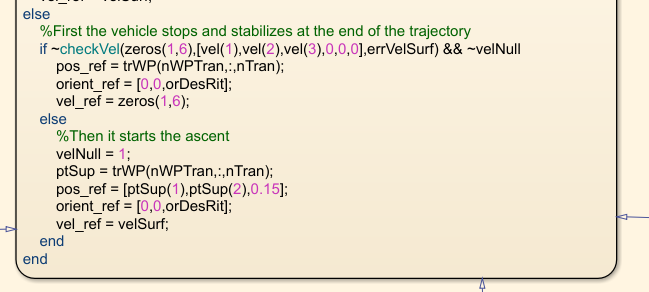
\includegraphics[scale = 0.3]{emer.png}}
                \label{fig:emer2}
            \end{figure}

            Una volta giunti nella condizione desiderata a meno di un certo margine di errore, avviene 
            la validazione della funzione presente nella condizione di transition da \emph{surfacing} a \emph{positioning}.\\
            Effettuato questo check, si setta $\emph{missionEnd} = 1$ (figura \ref{fig:missend} ), indicando appunto che 
            la missione è conclusa. In questo modo l'entry di \emph{positioning} setterà le variabili in uso di conseguenza.

            \begin{figure} [ht]
                \caption{Transizione di fine missione}
                \makebox[\textwidth]{
                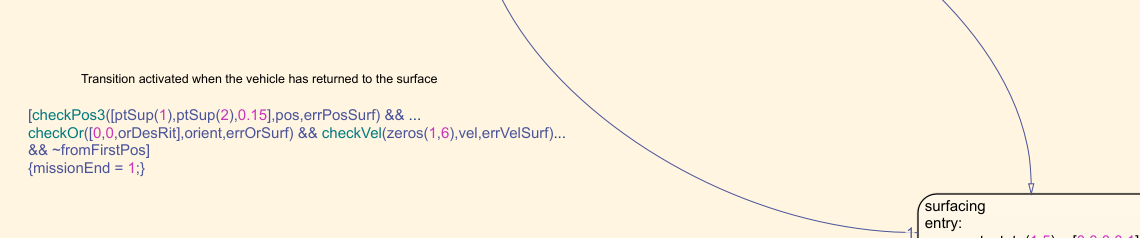
\includegraphics[scale = 0.3]{missend.png}}
                \label{fig:missend}
            \end{figure}

            Si entra infine nell'ultimo else in figura \ref{fig:else} dello stato, con il quale si forniscono riferimenti di posizione e orientazione di \emph{initPoint} 
            per ritornare al punto di deploy.

            \begin{figure} [ht]
                \caption{Gestione di positioning a fine missione}
                \makebox[\textwidth]{
                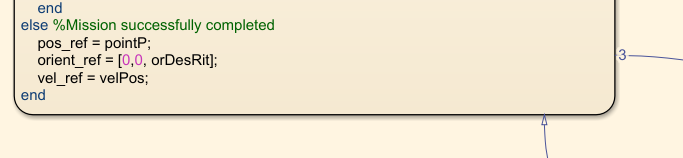
\includegraphics[scale = 0.3]{else.png}}
                \label{fig:else}
            \end{figure}

            E' presente dunque una sola transizione di uscita da \emph{surfacing} verso \emph{positioning}, proprio per ritornare al punto di partenza a fine missione.

            %\begin{figure} [ht]
            %    \caption{Blocco funzione di stop}
            %    \makebox[\textwidth]{
            %    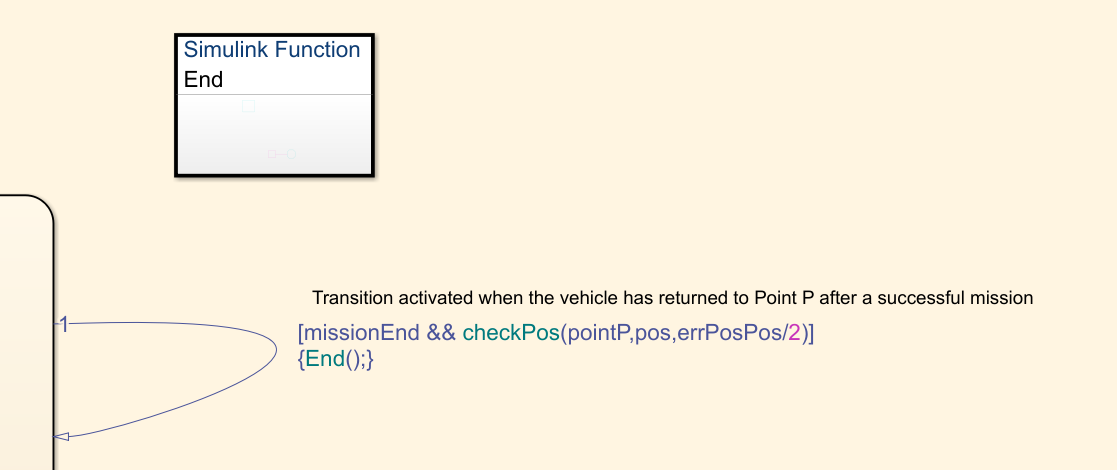
\includegraphics[scale = 0.3]{end.png}}
            %    \label{fig:end}
            %\end{figure}

            Anche in questo caso, per esser precisi, facciamo un check sulla posizione di arrivo: una volta che il veicolo è arrivato a riferimento, utilizziamo la funzione 
            di stop di figura \ref{fig:stop}
            per segnalare la fine della simulazione.

            \begin{figure} [ht]
                \caption{Funzione per terminare la simulazione}
                \makebox[\textwidth]{
                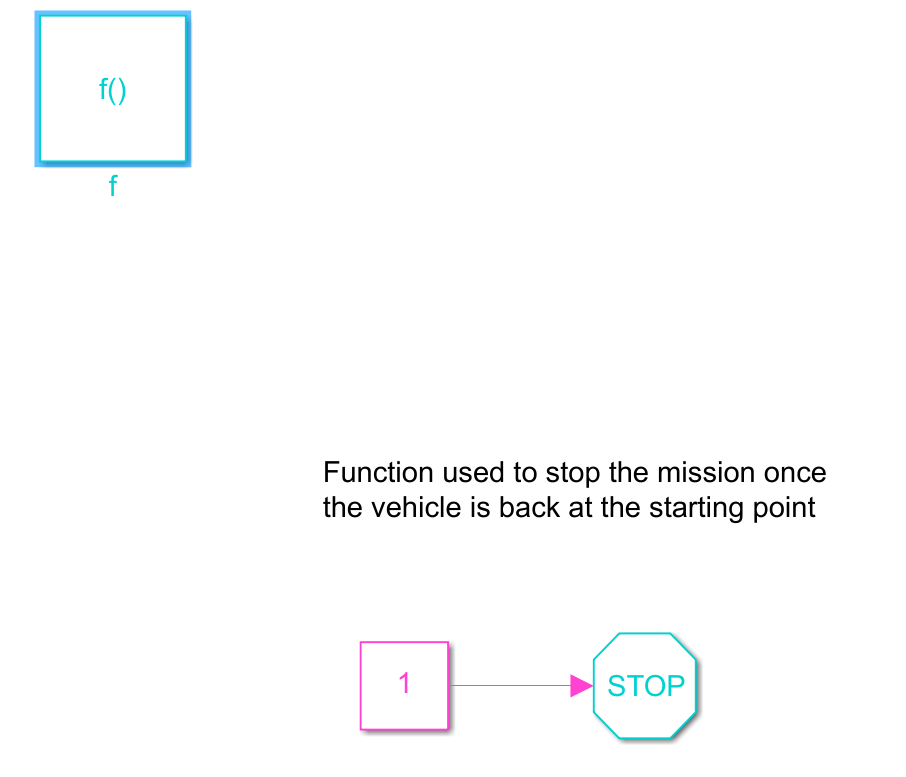
\includegraphics[scale = 0.3]{stop.png}}
                \label{fig:stop}
            \end{figure}

            \newpage
            
        \subsection{Implementazione del blocco Issues\_Management}

            \begin{figure} [ht]
                \caption{Subchart di Issues\_Management}
                \makebox[\textwidth]{
                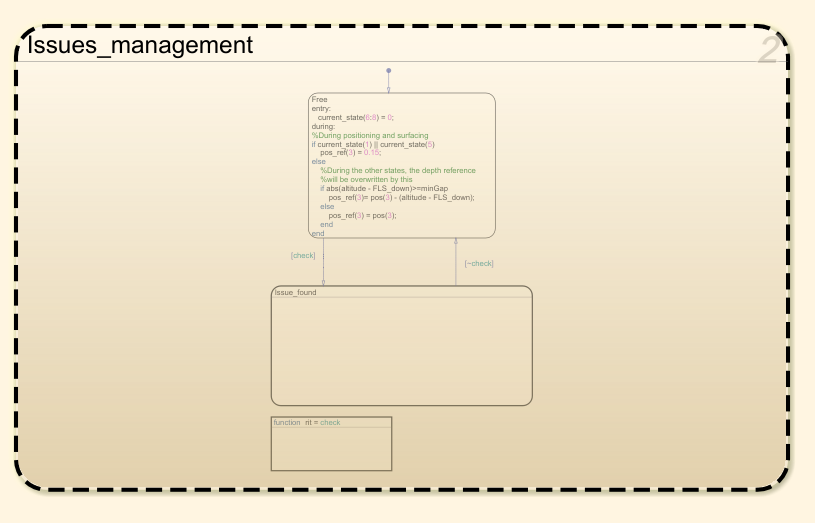
\includegraphics[scale = 0.3]{issman.png}}
                \label{fig:issman}
            \end{figure}

            Innanzitutto nel blocco generale di Issues vengono inizializzate due matrici vuote, \emph{points} e \emph{profs} (come si può notare in figura \ref{fig:iss} ), che definiremo in seguito.

            \begin{figure} [ht]
                \caption{Suddivisione di Issues\_Management in sottostati}
                \makebox[\textwidth]{
                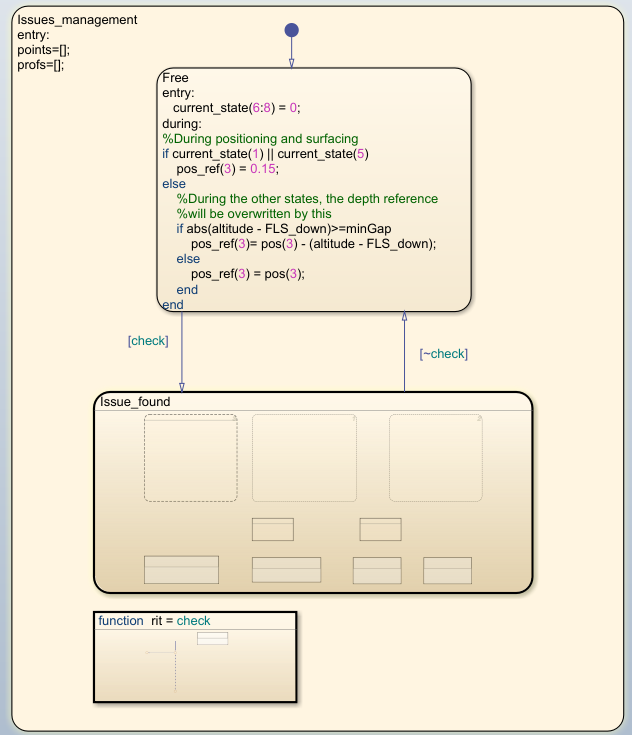
\includegraphics[scale = 0.3]{iss.png}}
                \label{fig:iss}
            \end{figure}

            All'interno del blocco la default transition, come spiegato precedentemente, è sul blocco \emph{Free} di figura \ref{fig:free} , che indica l'assenza di situazioni di emergenza
            e di conseguenza setta gli ultimi tre bit di \emph{current\_state} a 0.

            
            \begin{figure} [ht]
                \caption{Stato Free}
                \makebox[\textwidth]{
                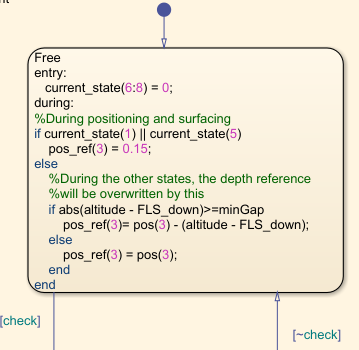
\includegraphics[scale = 0.3]{free.png}}
                \label{fig:free}
            \end{figure}

            E' in questo blocco che si fa il vero e proprio controllo del riferimento di profondità.\\
            Nel during, se \emph{current\_state} ha il bit in posizione 1 o 5 settato, vuol dire che siamo o nello stato \emph{positioning} o nello stato \emph{surfacing},
            dunque il riferimento di profondità di posizione è 0.15m; durante invece l'attivazione degli altri stati del blocco \emph{Movements}, 
            il riferimento di profondità sarà sovrascritto secondo la logica di base dell'implementazione della funzione di
            gestione ostacoli. Se la differenza (in termini di valori assoluti) tra il parametro costante \emph{altitude}, rappresentante il vincolo di profondità desiderata,
            e il parametro di distanza corrente da fondale è maggiore o uguale di 1m, allora andiamo a cambiare il riferimento di profondità; in caso contrario
            abbiamo ritenuto opportuno non modificare il riferimento di profondità in maniera tale da limitare la sensibilità
            del veicolo alle variazioni di un fondale molto irregolare.\\

            E' la funzione \emph{check} di figura \ref{fig:check} ad attivare la transizione dallo stato \emph{Free} al sottostato che supervisiona le condizioni di 
            emergenza \emph{warning, obstacle, abort}. 

            
            \begin{figure} [ht]
                \caption{Funzione check}
                \makebox[\textwidth]{
                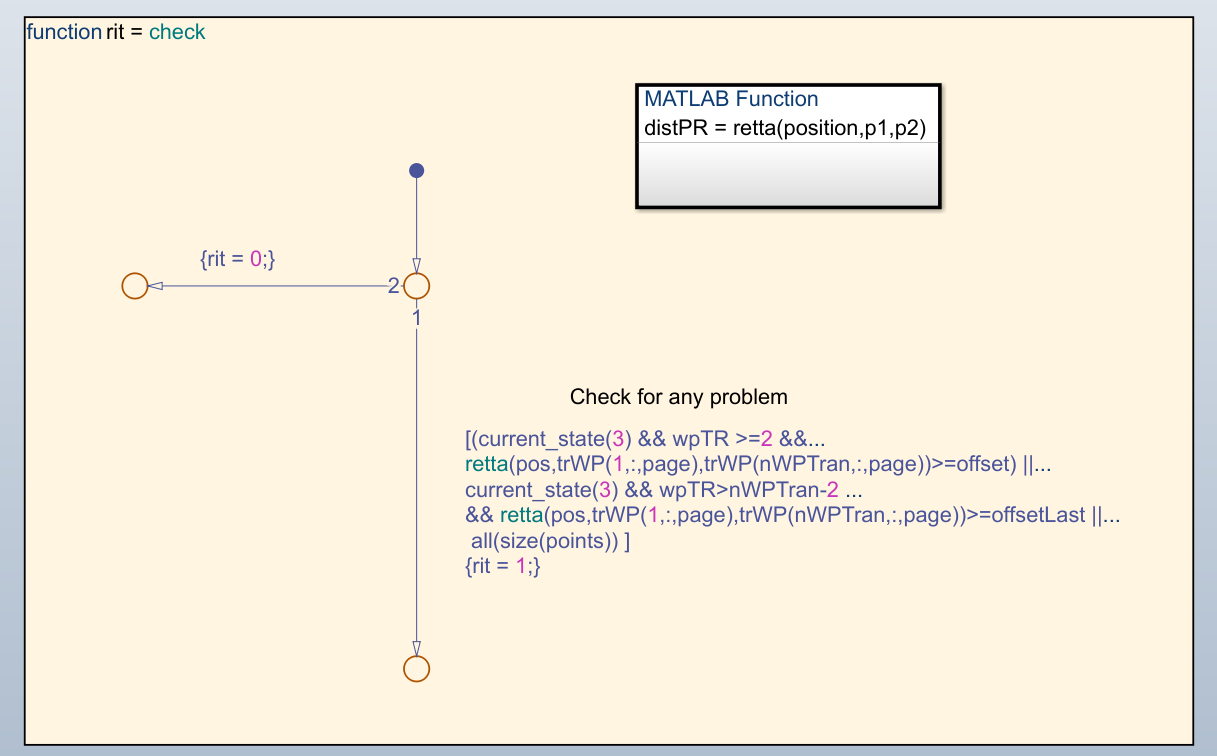
\includegraphics[scale = 0.3]{check.png}}
                \label{fig:check}
            \end{figure}

            Per verificare la possibile situazione di disallineamento si controlla che la distanza laterale del punto corrente
            rispetto alla retta del transetto di riferimento sia maggiore di un certo offset. Il controllo viene effettuato a partire dal secondo waypoint e non dal primo
            per consentire al veicolo di concludere la virata in maniera soddisfacente. La distanza laterale massima consentita è stata definita dalla variabile
            \emph{offset}, inizializzata a 2m.\\
            Nel caso in cui il disallineamento avvenga a partire dagli ultimi due waypoint,
            l'errore laterale massimo accettabile viene ridotto a 1m, perché in tali condizioni il veicolo ha solo pochi metri di transettaura per poter riallinearsi
            preventivamente alla fase di virata, quindi abbiamo optato per un trade-off di precisione ed effettiva capacità del veicolo.\\
            Nei casi in cui
            dunque si verificasse una delle situazioni di cui sopra, si esce dallo stato \emph{Free}, si attiva il sottostato relativo alla gestione delle emergenze,
            e il disallineamento sarà controllato dallo stato \emph{warning}.\\
            \\

            Il check che invece rileva la presenza di ostacoli viene effettuato controllando che il vettore \emph{points}, contenente i punti degli eventuali 
            ostacoli, non sia vuoto.
            \\
            \\Se non si è in nessuno dei casi sopra citati la funzione \emph{check} ritorna valore 0/false, quindi si
            rimane o si ritorna in \emph{Free}.\\

            
            Nel caso si verifichi il disallineamento, si entra nello stato \emph{warning} di figura \ref{fig:warn} e viene richiamata 
            la funzione \emph{disalignOP}: questa controlla se la distanza dal transetto supera l'offset da considerare e setta \emph{current\_state} con bit 1 in posizione 6.
            A seconda poi di quale stato è attualmente attivo in \emph{Movements} viene passato il riferimento di profondità corretto. 

            \begin{figure} [ht]
                \caption{Stato warning}
                \makebox[\textwidth]{
                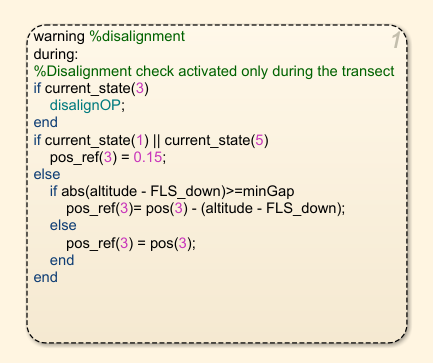
\includegraphics[scale = 0.3]{warn.png}}
                \label{fig:warn}
            \end{figure}

            La gestione del disallineamento viene effettuata nel blocco \emph{disaligned} di figura \ref{fig:dis} di transect, in \emph{Movements}.\\ 

            \begin{figure} [ht]
                \caption{Sottostato disaligned}
                \makebox[\textwidth]{
                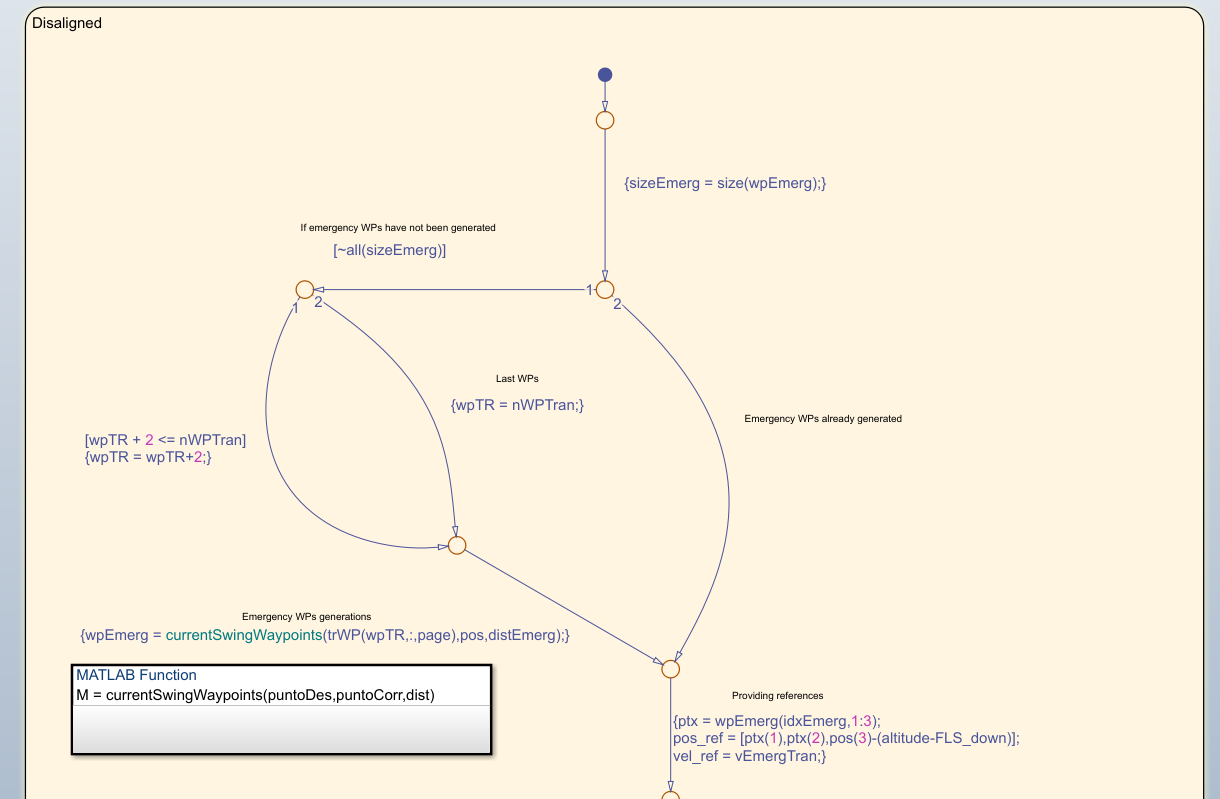
\includegraphics[scale = 0.3]{dis}}
                \label{fig:dis}
            \end{figure}

            Nella default transition si controlla il valore della lunghezza \emph{sizeEmerg} della matrice che contiene i waypoint d'emergenza (inizialmente vuota). 
            Se siamo appena entrati in condizione di disallineamento, non abbiamo ancora creato i midwaypoints di recupero traiettoria: di conseguenza, in base alla posizione
            attuale del veicolo si decide il punto a cui deve avvenire il riallineamento e si creano online i riferimenti necessari per ricondursi sulla traiettoria nominale desiderata.
            Normalmente tale punto finale viene deciso in maniera che sia ad almeno 5m dalla posizione corrente, ma in caso di disallineamento a fine transetto si fa in modo
            che il veicolo si riporti alla fine dello stesso, indipendentemente dalla posizione attuale.\\
            I punti d'emergenza vengono effettivamente creati tramite la chiamata alla funzione \emph{currentSwingWayPoints} in figura \ref{fig:emerg} .

            \begin{figure} [ht]
                \caption{Funzione currentSwingWayPoints}
                \makebox[\textwidth]{
                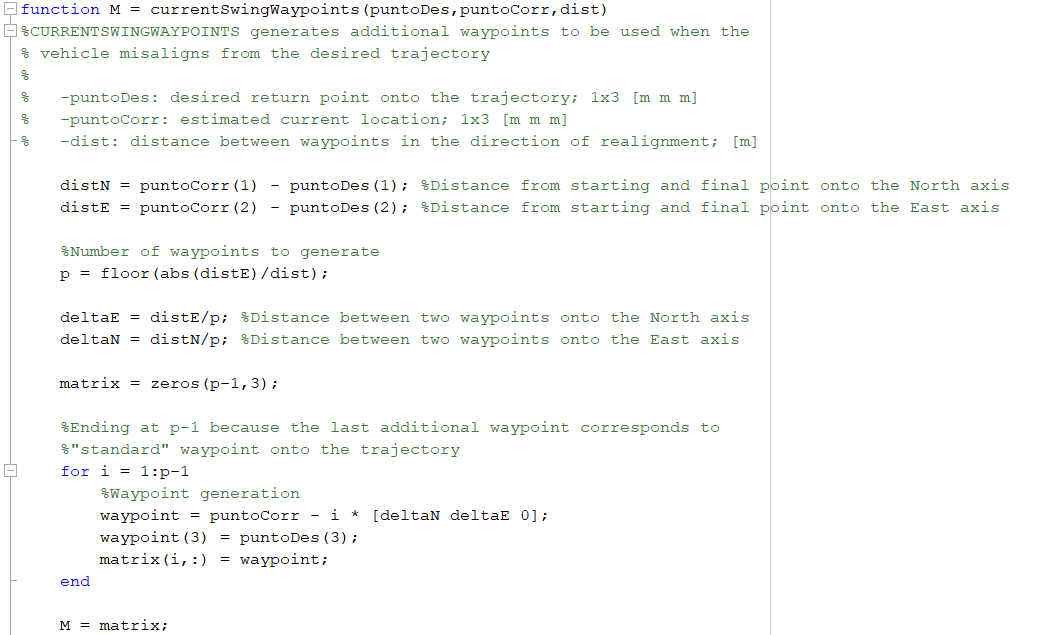
\includegraphics[scale = 0.3]{emerg.png}}
                \label{fig:emerg}
            \end{figure}

            In questa funzione si determina la distanza lungo la direzione Nord e lungo la direzione Est del punto corrente e di ritorno in traiettoria, si 
            divide tale distanza lungo Est secondo il parametro \emph{distEmerg}, settato a 0.5m, e si ottiene il numero di waypoints da generare.
            Successivamente si calcola la distanza lungo Nord e 
            lungo Est tra waypoints, in numero parametrico in base alla distanza dal punto di riallineamento. Quindi si popola la matrice relativa, avente numero di righe
            pari al numero dei waypoints generati meno 1, escludendo l'ultimo punto in quanto coincidente con l'effettivo riferimento sul transetto. 
            \\
            Il riferimento di orientazione fornito al blocco successivo rimane quello relativo all'orientazione desiderata sul transetto d'arrivo, mentre la velocità
            presenta valori minori per facilitare il recupero della condizione nominale.

            \begin{figure} [ht]
                \caption{Riferimenti forniti durante il disallineamento}
                \makebox[\textwidth]{
                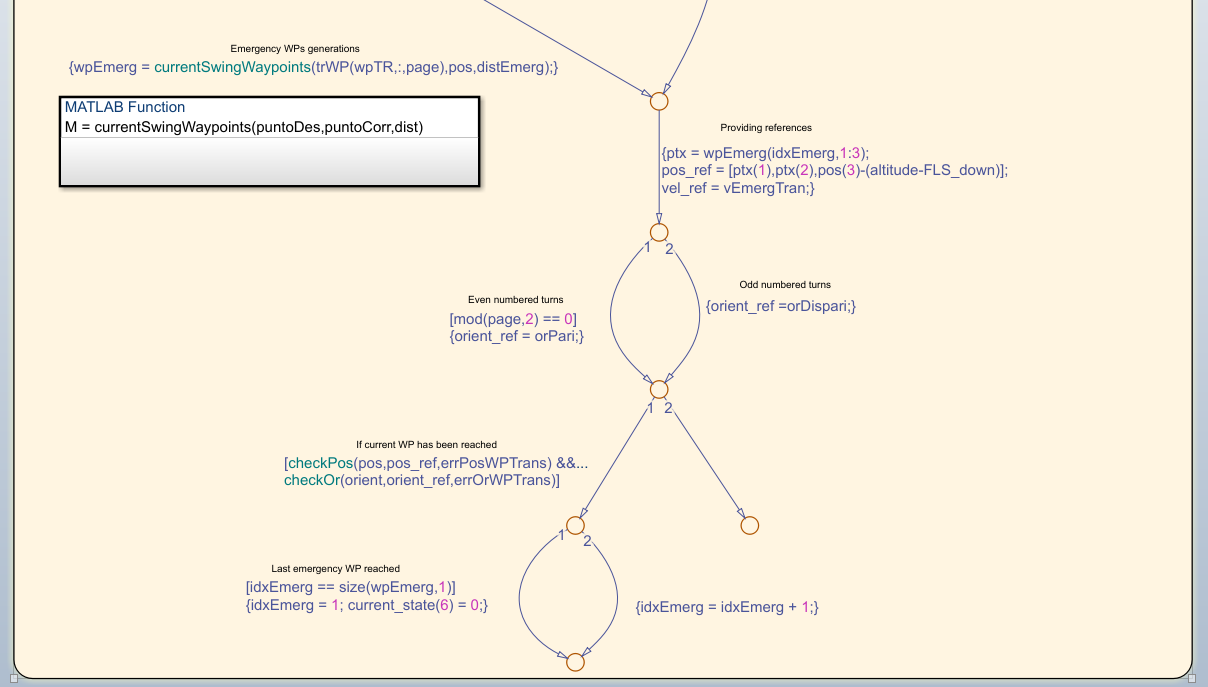
\includegraphics[scale = 0.3]{emerge.png}}
                \label{fig:emerge}
            \end{figure}

            Durante la fase di riallineamento abbiamo utilizzato
            margini di errore fra waypoint più stringenti, di 50cm sul surge e 20cm 
            su sway e heave, così da poter considerare tali riferimenti effettivamente raggiunti e fornire i riferimenti del punto successivo dopo aver attivato la transizione
            di figura \ref{fig:sx} .         

            \begin{figure} [ht]
                \caption{Transizione in caso di waypoint d'emergenza già creati}
                \makebox[\textwidth]{
                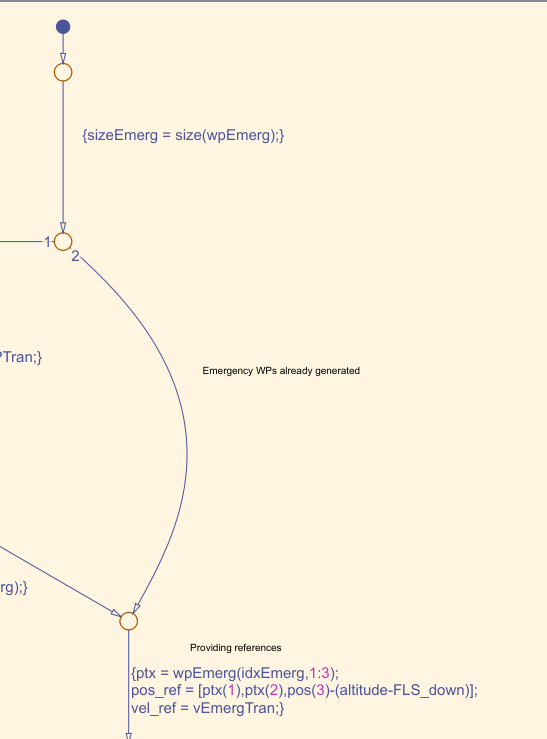
\includegraphics[scale = 0.3]{sx.png}}
                \label{fig:sx}
            \end{figure}

            Nel caso nel check venisse rilevata la presenza di ostacoli viene attivato lo stato \emph{obstacle} di figura \ref{fig:obs} .

            \begin{figure} [ht]
                \caption{Calcoli preventivi in obstacle}
                \makebox[\textwidth]{
                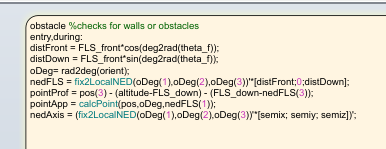
\includegraphics[scale = 0.3]{obs.png}}
                \label{fig:obs}
            \end{figure}

            Nell'entry e nel during di \emph{obstacle} si fa un calcolo che risulterà a noi comodo per poter poi effettuare la funzione di gestione dell'ostacolo.\\
            Sapendo già l'angolo di inclinazione del sonar frontale, possiamo calcolare, conoscendo lo slunt range del raggio, la lunghezza delle due proiezioni 
            lungo gli assi corpo del veicolo. La prima cosa che facciamo è riportare queste grandezze dal sistema di riferimento
            locale a quello globale tramite la funzione \emph{fix2LocalNED}, conoscendo l'orientazione corrente.\\
            \emph{pointProf} salva la profondità di riferimento sopra l'ostacolo rilevato: il primo termine in parentesi fa in modo che si tenga conto
            la differenza di profondità tra l'altitudine corrente dal fondale e quella desiderata, mentre il secondo termine nell'altra parentesi 
            considera la differenza tra la profondità corrente e quella di riferimento necessaria a superare l'ostacolo.\\
            \emph{pointApp} restituisce le coordinate North ed East del punto in cui è stato rilevato l'ostacolo. 
            \\
            Un importante accorgimento è stato quello di considerare che i valori di posizione durante la missione fanno riferimento al centro di massa del veicolo, quindi 
            si è reso necessario correggere le misure e le stime considerando anche i semiassi dell'AUV. Questa correzione non è banale, visto che il veicolo utilizzato
            presenta forma allungata con il semiasse in direzione di surge molto maggiore degli altri.

            \begin{figure} [ht]
                \caption{Valutazione di eventuale ostacolo dai nuovi dati ricevuti}
                \makebox[\textwidth]{
                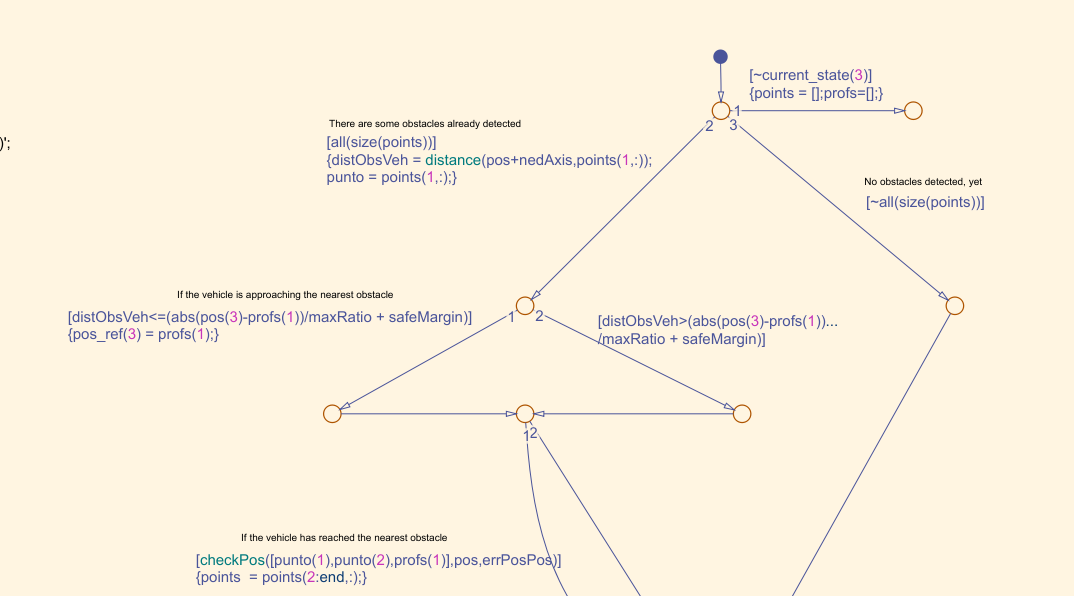
\includegraphics[scale = 0.3]{obs1.png}}
                \label{fig:obs1}
            \end{figure}

            Tramite giunzioni viene implementata la vera e propria funzione di gestione degli ostacoli: il primo controllo che si effettua tramite la default
            transition è quello che verifica se il veicolo sta già percorrendo un transetto, perchè si è deciso di attivare il controllo ostacoli solo in tale caso.\\
            Nella seconda transizione possibile si controlla che il vettore che contiene le coordinate North-East 
            dei punti con variazione di fondale rilevante non sia vuoto. In tal caso, è stata rilevata la presenza di un eventuale ostacolo da superare
            e tramite la funzione \emph{distance}
            viene calcolata la 
            distanza del veicolo rispetto a questo punto. Se siamo vicini all'ostacolo secondo una metrica che tiene conto delle performance del veicolo, il riferimento di profondità
            corrente verrà sovrascritto con un nuovo valore, utile a gestire la presenza dell'ostacolo sovracitato tramite la condizione in figura \ref{fig:ccond} .

            \begin{figure} [ht]
                \caption{Variazione del riferimento di profondità per superare l'ostacolo}
                \makebox[\textwidth]{
                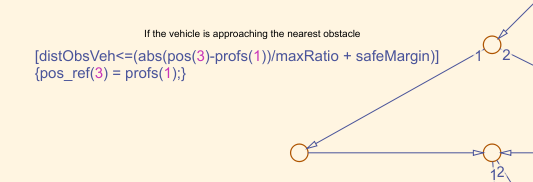
\includegraphics[scale = 0.3]{ccond.png}}
                \label{fig:ccond}
            \end{figure}

            Per spiegare la successiva condition e le variabili in essa utilizzate bisogna soffermarci su delle considerazioni preventive, alla base alla nostra politica di gestione
            degli ostacoli. Per prima cosa, grazie ai dati provenienti dal modulo \textit{Controllo}, sappiamo che il veicolo necessita di 8s di settling time per rispondere
            ad una variazione di profondità di 4m. La distanza necessaria per portarsi al nuovo riferimento di profondità, allora, varia a
            seconda della velocità a cui si sta muovendo il veicolo. \\
            Per prima cosa ci siamo dunque calcolati qual è la variazione massima di fondale che riusciamo a sostenere mantenendo il vincolo di profondità costante, con la 
            relativa distanza minima necessaria per tale spostamento. 
            Per considerazioni ulteriori di sicurezza (presenza di forti correnti, errori di misura, limitazioni fluidodinamiche...), abbiamo deciso 
            di moltiplicare per 2 il valore di distanza orizzontale di cui il veicolo avrebbe bisogno per superare l'ostacolo. Dal momento che il veicolo è equipaggiato
            con un sonar inclinato di $45\degree$, sappiamo la
            distanza veicolo-ostacolo lungo l'asse di surge a cui iniziamo a rilevare la variazione di fondale. Quindi, tramite il confronto del rapporto tra la
            variazione di profondità rilevata e la distanza da coprire durante tale gap, e dello stesso rapporto di riferimento in condizioni ideali \emph{maxRatio}, possiamo
            stabilire se il veicolo riuscirà effettivamente a superare l'ostacolo. Il tutto viene calcolato come in figura \ref{fig:consid} .

            \begin{figure} [ht]
                \caption{Dati di riferimento per il superamento degli ostacoli}
                \makebox[\textwidth]{
                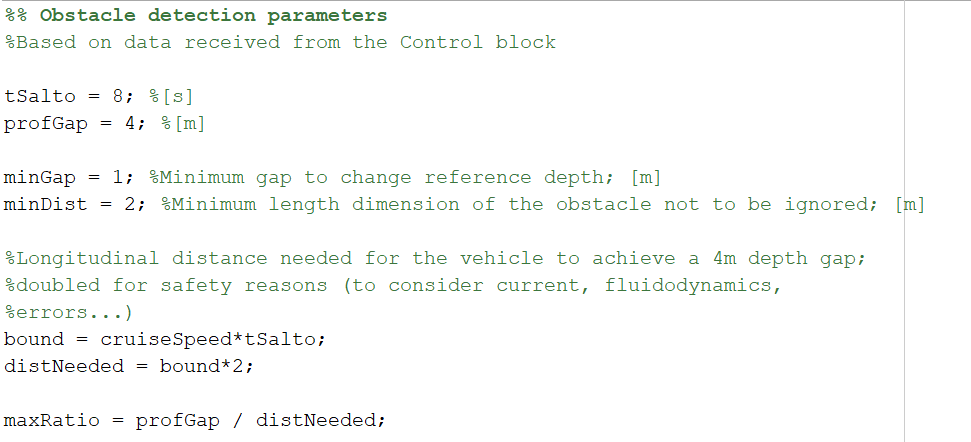
\includegraphics[scale = 0.3]{consid.png}}
                \label{fig:consid}
            \end{figure}

            Dopo tutte queste considerazioni, verrà ora spiegato come e quando viene passato al modulo \textit{Controllo} il riferimento di cambiamento di profondità.\\
            \\
            Tramite la differenza di $pos(3) - profs(1)$ in figura \ref{fig:obs2} , conosciamo quanto è la variazione 
            effettiva della profondità del fondale rispetto alla situazione corrente. La dividiamo per il valore di \emph{maxRatio} è otteniamo una stima della distanza
            necessaria al veicolo per il superamento dell'ostacolo, a cui viene sommato un ulteriore margine di sicurezza \emph{safeMargin}.\\
            \\
            La condition sull'arco successivo indica poi che se la distanza tra la posizione corrente del veicolo e l'ostacolo è maggiore rispetto a 
            quella che effettivamente serve per posizionarsi sopra di esso, non viene cambiato il riferimento di profondità e il 
            veicolo non attua nessuna variazione di altitudine; in caso contrario, il riferimento viene cambiato in maniera da far cominciare al veicolo la manovra necessaria.

            
            \begin{figure} [ht]
                \caption{Valutazione avvicinamento del veicolo all'ostacolo}
                \makebox[\textwidth]{
                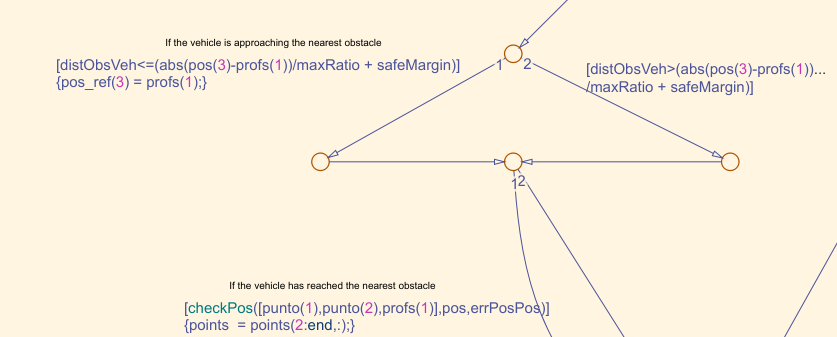
\includegraphics[scale = 0.3]{obs2.png}}
                \label{fig:obs2}
            \end{figure}

            Successivamente, come mostrato ancora nella figura \ref{fig:obs2} , si fa un check per assicurarsi di essersi portati sopra l'ostacolo con vincolo di altitudine 
            rispettato. Se il check va a buon fine, viene modificato il vettore contenente le coordinate degli ostacoli eliminando il primo elemento, relativo all'ostacolo 
            appena superato.

            \begin{figure} [ht]
                \caption{Rilevazione ostacolo compromettente la missione}
                \makebox[\textwidth]{
                \includegraphics[scale = 0.3]{wall1.png}}
                \label{fig:wall1}
            \end{figure}

            Fintanto che il punto non è stato raggiunto, e per ogni nuovo dato ricevuto, si fa un check molto importante rappresentato in figura \ref{fig:wall1} : se il rapporto tra variazione di 
            profondità rilevata e distanza necessaria è maggiore del rapporto ideale \emph{maxRatio}, vuol dire che non abbiamo lo spazio necessario lungo l'asse di
            surge per superare l'ostacolo, quindi viene aggiornato \emph{current\_state} per segnalare la presenza di parete (settimo bit), andando quindi a far attivare
            lo stato di riemersione. 

            
            \begin{figure} [ht]
                \caption{Valutazione nuovo oggetto scansionato}
                \makebox[\textwidth]{
                \includegraphics[scale = 0.3]{nopieno.png}}
                \label{fig:nopieno}
            \end{figure}

            Nel caso in cui invece siamo in condizioni favorevoli per il superamento dell'ostacolo, si verifica se il vettore \emph{points} ha degli elementi.
            \\
            Se esso è vuoto (figura \ref{fig:nopieno} ), si controlla solo che la differenza tra la profondità corrente e quella relativa 
            a \emph{pointProf} sia maggiore di 1m e che la distanza ostacolo-veicolo sia maggiore di $\emph{minDist} =  2m$: in tali condizioni, l'oggetto rilevato viene effettivamente
            considerato come un ostacollo da superare, assimilabile all'esempio di figura \ref{fig:ostacoli} , e conseguentemente gestito.


            
            \begin{figure} [ht]
                \caption{Confronto nuovo ostacolo con altri già rilevati}
                \makebox[\textwidth]{
                \includegraphics[scale = 0.3]{pieno.png}}
                \label{fig:pieno}
            \end{figure}

            In caso contrario,
            si effettuano i controlli finora descritti anche per valutare la presenza di una variazione eccessiva di profondità tra due ostacoli successivi, precisamente
            tra quello appena rilevato e l'ultimo considerando rilevante e quindi presente in \emph{points}. Una situazione simile, come evidenziato in figura \ref{fig:pieno} ,
            porterebbe il veicolo a superare il primo ostacolo (tra i due considerati), ma comprometterebbe dopo di esso la continuazione e terminazione della missione,
            segnalando al veicolo di portarsi in superficie. \\
            Per evitare tale comportamento si è scelto di violare solo in questo caso il vincolo di altitudine costante dal fondale, per consentire al veicolo di ignorare il
            primo ostacolo e muoversi subito in maniera utile a superare anche il secondo, così da poter poi continuare la missione.

            
            \begin{figure} [ht]
                \caption{Esempio di scansione di un ostacolo}
                \makebox[\textwidth]{
                \includegraphics[scale = 0.3]{ostacoli.png}}
                \label{fig:ostacoli}
            \end{figure}
        
    \section{Conclusioni e possibili sviluppi futuri}
        Dopo aver effettuato una serie di prove e simulazioni sulla nostra macchina a stati integrata con tutti gli altri moduli, abbiamo 
        verificato e possiamo concludere che il lavoro di \textbf{\textit{missionSupervisor}} è stato portato a termine con successo. \\
        La nostra sfida è stata quella di misurarci con 
        lavoro di grandi dimensioni in ambiente MATLAB/Simulink con utilizzo di Stateflow (quest'ultimo del tutto nuovo per noi), favorendo un arricchimento delle nostre 
        competenze.\\
        
        \subsection{Considerazioni a livello implementativo}
            La prima fase di lavoro ci ha parecchio impegnato per decidere nella maniera più ottimale e ragionevole possibile,
            i task principali della missione, per determinare perlomeno a grandi linee la politica di gestione di tutto il task e successivamente sviluppare i singoli
            macrotask delle varie operazioni da compiere.\\ 
            A tal proposito i confronti tempestivi durante le lezioni e con il nostro referente sono stati fondamentali, per un 
            indirizzamento verso determinate scelte gestionali e implementative piuttosto che altre.\\
            Essendo stata per tutto il gruppo la prima volta in cui ci si è 
            trovati a dover sviluppare un lavoro di tipo progettuale all'interno di un team, avere un feedback pressocché costante sotto tale aspetto, 
            è stato di fondamentale importanza.\\
            E' stato il lavoro delle ultime settimane ad essere più oneroso, perché quando abbiamo dovuto testare le prime integrazioni con tutti i blocchi abbiamo incontrato 
            diversi stalli. Le prime 'discordanze' si sono verificate col blocco \textit{Controllo}, che ha preferito una suddivisione dei task a livello molto più elementare
            rispetto a quanto avevamo precedentemente stabilito. In tal 
            caso siamo stati subito attivi e disponibili nel modificare la politica di gestione e il relativo codice all'interno della nostra macchina a stati e nei singoli blocchi
            interessati. Sotto richiesta abbiamo anche modificato la politica di gestione delle virate, poiché il controllo ha preferito un approccio di tipo temporizzato,
            che noi avevamo personalmente scartato.\\
            Modificato tutto ciò, in una prima fase i test sono stati effettuati solo in condizioni nominali, ossia in assenza di correnti e di situazioni di emergenza, quali
            ostacoli e disallineamenti.
            Superate con successo tali prove, il secondo 'stallo' che ci si è presentato, è stato quello dell'integrazione del codice ostacoli, che era poi la base del compimento
            del nostro task. Nonostante 
            avessimo tutto pronto, non abbiamo potuto testare ciò che si era implementato, poichè inapplicabile a causa di miglioramenti richiesti ma non tempestivamente apportati ai
            moduli \emph{Controllo}
            e \emph{Modello}. Grazie ad un successiva riunione con il professore, il tutto si è sbloccato, i gruppi si sono mossi nella direzione giusta
            e siamo stati così capaci di validare e verificare l'implementazione del nostro codice.\\
            A tal proposito le prove che abbiamo effettuato hanno riguardato:
            \begin{itemize}
                \item survey con lato maggiore lungo Nord e lungo Est; \\
                \item angolo $\alpha$ di orientazione differente; \\
                \item distanza tra transetti maggiore e minore;\\
                \item riferimento di altitudine diverso;\\
                \item velocità di crociera diverse, fino a 2 m/s;\\
                \item corrente di diverse incidenze;\\
                \item diversi \emph{initPoint} e  \emph{surveyAreacorner}.\\
            \end{itemize}
            
            
            Per quanto riguarda gli eventuali sviluppi futuri, sono state diverse le situazioni che abbiamo tenuto in considerazione.\\   
            Si è pensato, nei casi in cui le elevazioni da fondale fossero molto più importanti, di poter utilizzare dei sonar meno inclinati in maniera tale da aumentare 
            lo slunt range utile e dunque
            l'anticipo sugli ostacoli.\\
            Altra alternativa per risolvere tale problematica può essere far partire il veicolo ad una
            distanza (orizzontale o verticale) maggiore dal punto inizio survey, così da poterlo far partire con più metri di anticipo su eventuali variazioni importanti del fondale.\\
            \\
            Una migliorìa che si può aggiungere al codice riguarda la gestione del disallineamento: per disallineamenti importanti sarebbe più consono, per un veicolo di forma allungata 
            quale il nostro, evitare moti traslazionali laterali e prevedere invece un'imbardata nella direzione di
            riallineamento prima di dirigersi verso il transetto, per permettere all'AUV di muoversi principalmente con moto di surge, più adatto per il modello utilizzato.
            \\
            Nel nostro caso non subiamo 
            disallinemaneti importanti, quindi il veicolo riesce a riportarsi senza problemi in traiettoria con moto traslazionale.\\
            Un'ultima constatazione che si è fatta è stata la possibilità di aumentare e gestire diversi casi in cui la missione deve passare nello stato 
            di abort: alcuni esempi possono essere la ricezione misure sbagliate per malfunzionamenti dei sensori, livelli di batterie che non riescono a portare 
            a termine il task, situazioni ambientali estreme...

        \clearpage
        \listoffigures
        \newpage
        \printbibliography
\end{document}

